\chapter{Contrasting effects of convective intensity and organisation on the structure and lifecycle of \acrshort{dcc}s} \label{chp:anvil_structure}

\section{Introduction}

Understanding how the structure of anvil clouds changes in response to changes in convective behaviour is vital to understanding the radiative impacts and climate feedbacks of \acrshort{dcc}s.
Around 50\% of cirrus clouds in the tropics originate from deep convection \citep{massie_distribution_2002, luo_characterizing_2004}.
Overall, anvil clouds have a near-neutral radiative impact on the tropics, despite their large \acrshort{sw} reflectance and \acrshort{lw} absorption \citep{hartmann_effect_1992, hartmann_tropical_2016}.
Their radiative effect is not homogeneous however; while the optically thick portion of anvil clouds generally have a cooling effect at the \acrshort{toa}, the thin, detrained cirrus has a strong warming effect \citep{berry_cloud_2014}.
As a result, changes in convective activity that result in a change in the size and structure of anvil clouds may have large impacts on the climate.

The change of anvil cloud area in response to warming---the iris effect \citep{lindzen_does_2001, bony_thermodynamic_2016}---is generally considered to have a cooling feedback in response to climate change.
However, it is the largest source of uncertainty in cloud--climate feedbacks, with around a third of models predicting a warming response \citep{sherwood_assessment_2020}.
To address this uncertainty, a better understanding of the links between convective processes and anvil properties, changes in anvil structure and the properties of ice clouds are required \citep{gasparini_opinion_2023}.

Assessing the extent of thin anvil cirrus is challenging due to the difficulties in observing these clouds using \acrshort{ir} radiometers.
The low emissivity of thin cirrus clouds means that observed \acrshort{bt} is dominated by radiances from the lower atmosphere and surface below.
\citet{protopapadaki_upper_2017} used cloud emissivity and cloud top pressure, rather than \acrshort{bt}, to detect convective cores, thick and thin anvil cirrus clouds.
Data from the AIRS instrument was used to retrieve these emissivity values, as the hyperspectral sounder is more sensitive to thin cirrus than \acrshort{ir} radiometers.
They then compared the proportion of each anvil cloud consisting of thin anvil to the minimum observed cloud top temperature within the convective core, a proxy for the convective depth which is, in turn, a proxy for convective intensity.
It was found that the thin cirrus anvil proportion increased with colder cloud top temperatures, indicating that stronger convection increases the detrainment of thin cirrus.

\citet{takahashi_relationships_2017} built upon this study using collocated measurements from the \acrfull{cpr} aboard CloudSat.
The \acrshort{cpr} measurements provide the echo top height, measuring the convective depth directly, and also provide another proxy for convective intensity, the echo top distance, which is independent of convective depth \citep{takahashi_characterizing_2014}.
It was again found that the proportion of thin cirrus increased with the echo top height, and also increased with decreasing echo top distance (indicating stronger convection).

It should be noted that both of these studies were performed using observations from polar-orbiting satellites in the A-train, and so do not fully sample the diurnal cycle.
While both studies consider the maturity of the \acrshort{dcc}s observed, the thin anvil proportion is measured at a single point in time, and so differences in the lifetime of the thick and thin anvil cirrus are not considered.
It is expected that the structure of an anvil will change over its lifetime, with the thin anvil fraction increasing as the anvil dissipates.
However, the observed \acrshort{bt} of the anvil also changes over its lifetime \citep{futyan_deep_2007}, and so the use of \acrshort{bt} as a proxy for convective intensity is not an independent measurement.
While the use of echo top height avoids this confounding issue, these collocated measurements can only be made when the \acrfull{dcc} is convectively active and so cannot be used to assess the structure of dissipating anvils.

Chapter~\ref{chp:lifecycle} presented a large dataset of tracked \acrshort{dcc}s, including growing cores, and thick and thin anvils, and showed that this dataset captures relations between convective processes and anvil properties.
By using geostationary satellite observations changes in the structure of \acrshort{dcc} anvils can be investigated throughout their lifecycles, along with changes in the lifetime of both thick and thin anvils.
Furthermore, the impacts of convective organisation on anvil structure can be investigated by taking into account the number of cores associated with each anvil.


\section{Data}

The dataset of tracked \acrshort{dcc}s first presented in chapter~\ref{chp:lifecycle} is utilised here to investigate how the structure of observed \acrshort{dcc}s depends on the properties of their convective cores.
Produced using the method detailed in chapter~\ref{chp:tracking_method}, convective cores are tracked during their vertically growing period, and thick and thin anvils are subsequently tracked using two different channel combinations.
Changes in the proportion of thick and thin anvil coverage, considering both spatial extent and the lifecycle of the anvil cloud, can be investigated.

Data filtering is applied to detected anvils according to the criteria shown previously in table~\ref{table:anvil_validity_criteria}.
This results in a total of 391,050 anvils considered for analysis, which between them are connected to a total of 792,522 cores.
The filtering requires that every anvil in the analysis dataset begins with a valid observed core, ensuring that the subsequent development of the anvil can be linked to the properties of the core.
In addition, it ensures that each anvil is observed for its entire lifetime, and the entire extent of both thick and thin anvil are observed over this period.
While this does mean that fewer large anvils are considered valid as their greater extent means that they are more likely to intersect the edges of the domain, it ensures that changes in both thick and thin anvil area can be considered robust over the entire lifecycle of the analyses anvils.

The dataset contains a range of properties relating to the observed \acrshort{dcc}s.
This chapter will focus on how the area of the detected cores, thick and thin anvils change with each time step.
Two related properties are also analysed; the maximum area of the thick and thin anvil, i.e.\ the area at the time step when the anvil reaches its maximum observed extent, and the total area which is the sum of the areas observed at each time step over each anvils lifetime.
The thin anvil proportion refers to the area of the detected thin anvil divided by the total area of both anvil and core.
In general, this is calculated as the total over the entire \acrshort{dcc} lifetime, although section~\ref{sec:composite_results} will investigate how this changes over the \acrshort{dcc} lifecycle.

There is additional consideration on how the \acrshort{bt} of each core and anvil change over time.
The area-weighted average of the 10.4\,\unit{\mu m} \acrshort{bt} is taken at each time step for each core, thick and thin anvil.
The 10.4\,\unit{\mu m} \acrshort{lw} window \acrshort{bt} has a minimal contribution from water in the atmosphere, and so can provide temperature measurements of clouds from near the surface to the top of the atmosphere.
It should be noted that the \acrshort{bt} is affected by the emissivity of the cloud, and so for thin cirrus the observed \acrshort{bt} will be warmer than the actual \acrshort{ctt} due to the contribution from the atmosphere below.
As a result, the mean \acrshort{bt} of the thick anvil is used as a proxy for convective cloud height as this avoids a bias from the warmer thin anvil.
The (negative) cooling rate of each core is calculated as the largest change in the mean core \acrshort{bt} measured over any 15-minute period.
This relates to the vertical growth of the \acrshort{dcc} core as discussed in section~\ref{sec:theory_core}, with a cooling rate of 1\,K$\cdot\mathrm{minute^{-1}}$ corresponding to a vertical growth rate at the cloud top of 2.5\,$\mathrm{ms^{-1}}$.

\section{Method}

\subsection{Detection of thick and thin anvils}

Observing thin cirrus anvils using satellite \acrshort{bt} is difficult due to their low emissivity.
Furthermore, \acrshort{bt} is affected both by the height of the observed cloud and its optical thickness.
As shown in fig.~\ref{fig:optical_depth_channels}, the observed \acrshort{bt} increases as optical depth decreases.
For detection using a fixed threshold, as used in many anvil detection algorithms, this means that the limit of optical depth at which the anvil is detected increases as the height of the cloud decreases.
This results in the detected anvil area varying with height, with an anvil at a lower altitude being detected as smaller than one at a higher altitude even if there size and structure are otherwise identical.
This problem with detected anvil area using \acrshort{bt} thresholds was identified as early as \citet{augustine_mesoscale_1988}, but remains a feature of many detection algorithms to this day (see e.g.\ section~\ref{sec:tracking_timeline}).

%f
\begin{figure}[tp]
    \centering
    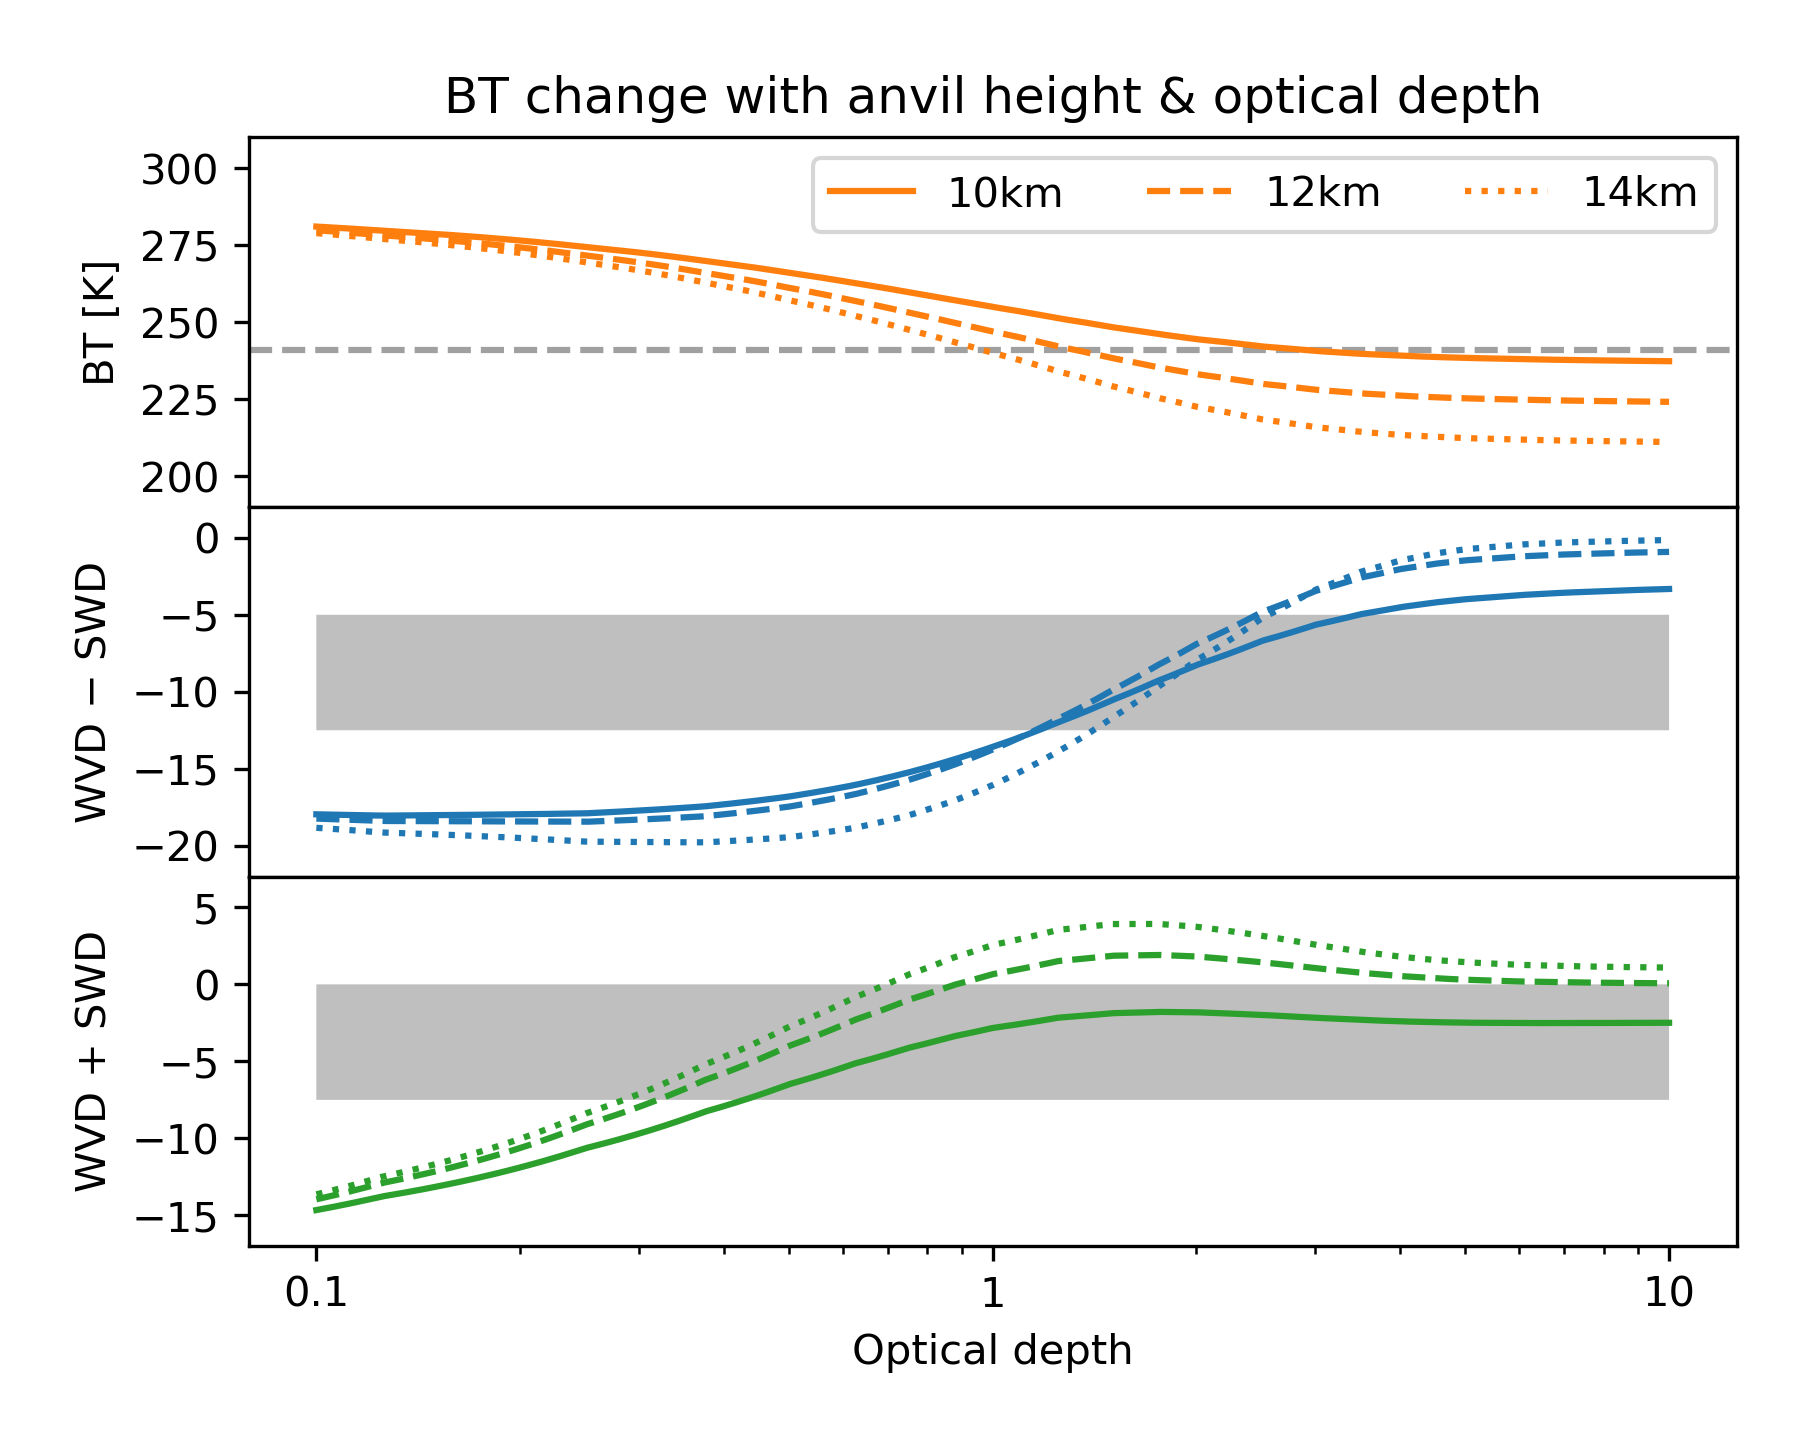
\includegraphics[width=0.9\textwidth]{figures/chapter3_01.png}
    \caption[
    Simulated \acrshort{abi} \acrshort{bt} observations of \acrshort{dcc} anvils at a range of heights and optical depths for detection of thick and thin anvil detection
    ]{
    Simulated \acrshort{abi} \acrshort{bt} observations for \acrshort{dcc} anvils at 10\,\unit{km} (solid lines), 12\,\unit{km} (dashed lines) and 14\,\unit{km} (dotted lines) at optical depths between 0.1 and 10. Panels show (top) 10.4\,\unit{\mu m} \acrshort{bt}; (middle) \acrshort{wvd} minus \acrshort{swd}, used in thick anvil detection; and (bottom) \acrshort{wvd} plus \acrshort{swd}, used in thin anvil detection. The grey dashed line shows the 241\,\unit[K] threshold, and the grey shaded regions show the range in which cloud edge detection is performed for thick and thin anvils.
    }
    \label{fig:bt_wvd_swd_height_od}
\end{figure}

While observing the thin cirrus anvil is challenging, section~\ref{sec:anvil_detection} showed that thin anvil cirrus can be detected using a combination of the \acrshort{wvd} and \acrshort{swd} differences from \acrshort{abi}.
Furthermore, the use of channel differences reduces the height dependence of the detection of anvils compared to the use of a single \acrshort{bt}.
Figure~\ref{fig:bt_wvd_swd_height_od} shows simulated \acrshort{bt} observations using the libRadTran model \citep{emde_libradtran_2016}, as described in section~\ref{sec:detection_theory}.
The top panel shows simulation \acrshort{bt} observations by \acrshort{abi} at 10.4\,\unit{\mu m} at heights of 10, 12 and 14\,\unit{km} (shown by the solid, dashed and dotted lines respectively).
Also shown by the grey, dashed line is an example of the 241\,\unit{K} \acrshort{bt} threshold.
At this threshold there is substantial variance in the limit of \acrshort{od} at which anvil clouds are detected, which ranges from 1 at 14\,\unit{km} to 3 at \unit{km}.
This provides clear support for the argument made by \citet{augustine_mesoscale_1988} that the anvil area detected using this threshold is ``subjective''.

The middle and bottom panels in fig.~\ref{fig:bt_wvd_swd_height_od} show the simulated \acrshort{od} for the combinations of \acrshort{wvd} minus \acrshort{swd} and \acrshort{wvd} plus \acrshort{swd} respectively.
Section~\ref{sec:anvil_detection} describes how these two channel combinations are used for the detection of thick and thin anvils.
In both panels, the grey shaded region shows the \acrshort{bt} range in which edge detection is used to find the anvil area.
Compared to 10.4\,\unit{\mu m} \acrshort{bt}, the \acrshort{wvd} minus \acrshort{swd} combination shows very little variance in the optical depths at which the anvil cloud is detected within the threshold range.
Throughout the threshold range of --5 to --12.5\,\unit{K} the \acrshort{od} corresponding to the same observed \acrshort{bt} difference varies by approximately 0.1--0.2 between differing heights, compared to 1--2 for 10.4\,\unit{\mu m} \acrshort{bt}.

The \acrshort{wvd} plus \acrshort{swd} combination is shown in the bottom panel of fig.~\ref{fig:bt_wvd_swd_height_od}.
Greater variance between different heights is seen, particularly for the 10\,\unit{km} anvil simulation.
However, the \acrshort{od} corresponding to the observed \acrshort{bt} differences are very similar throughout the detection range of 0 to --7.5\,\unit{K} for heights of 12 and 14\,\unit{km}.
Lidar observations of thin cirrus anvil have shown that the heights of these clouds typically exceed 12\,\unit{km} \citep{wall_observational_2020, horner_evolution_2023}, and so little difference is expected in the sensitivity to observed anvils.

It should be noted that the simulations shown in fig.~\ref{fig:bt_wvd_swd_height_od} were calculated using a standard tropical atmospheric profile to best represent the moist environment in which deep convection occurs.
While anvils occurring in the extra-tropical parts of the \acrshort{conus} domain are expected to have lower cloud top heights, there is also expected to be a colder temperature profile.
As a result, the observed \acrshort{bt} of extra-tropical \acrshort{dcc}s behave more like that of the 12 and 14\,\unit{km} simulations shown in fig.~\ref{fig:bt_wvd_swd_height_od}, rather than that at 10\,\unit{km}.


\subsection{Estimation of convective intensity and organisation} \label{sec:method_proxies}

As the vertical velocity or convective mass flux of \acrshort{dcc} updrafts cannot be obsered directly using geostationary satellite observations, a proxy is needed to estimate their intensity instead.
The minimum \acrshort{bt} of an observed \acrshort{dcc} is commonly used as a proxy for convective intensity, and is used by \citet{protopapadaki_upper_2017} for this purpose.
This property is more closely related to the height of the \acrshort{dcc}, however.
While the height of a \acrshort{dcc} is related to the intensity of convection, it is also related to the tropopause height and level of neutral buoyancy which may vary with location and meteorology independent of convective processes.
While the minimum \acrshort{bt} of observed anvils in this chapter to better compare to previous studies, a more direct proxy for convective intensity is desired.

The primary proxy for convective intensity in this chapter is the maximum cooling rate of the initial observed core for each \acrshort{dcc}.
As described in section~\ref{sec:theory_core}, the core cooling rate is linked to the vertical development of the core over time.
A cooling rate of 1\,\unit{K minute\textsuperscript{-1}} approximately represents a cloud top vertical velocity of 2.5\,\unit{ms\textsuperscript{-1}}.
While this should not be confused with the updraft velocity of the core itself, and is expected to be less due to the effects of entrainment and overturning circulation at the top of the updraft, it is linked to the updraft velocity directly.
In section~\ref{sec:core_properties} it was shown that the core cooling rate and minimum core \acrshort{bt} are correlated.
The maximum cooling rate of an anvil is measured on the initiating core to ensure that there are sufficient observations of the core throughout its growth that are not masked by an anvil above.
While the updraft may strengthen later in the development of the \acrshort{dcc}, or subsequent cores in a multi-core system have stronger updrafts, this is considered the most direct and robust proxy available for the updraft intensities of \acrshort{dcc}s observed by geostationary satellites.

The number of cores associated with each \acrshort{dcc} is used as a measure of its organisation, again providing the most direct proxy available.
While it may not be possible to observe all the cores associated with larger \acrshort{mcs}s due to the anvil blocking observations of cores below, it is still expected that many separate cores associated with such systems are detected.
As shown in chapter~\ref{chp:lifecycle}, tracked \acrshort{dcc}s with many cores show the properties expected of \acrshort{mcs}s.


\subsection{Lifecycle analysis} \label{sec:lifecycle_definition}


\begin{figure}[tp]
    \centering
    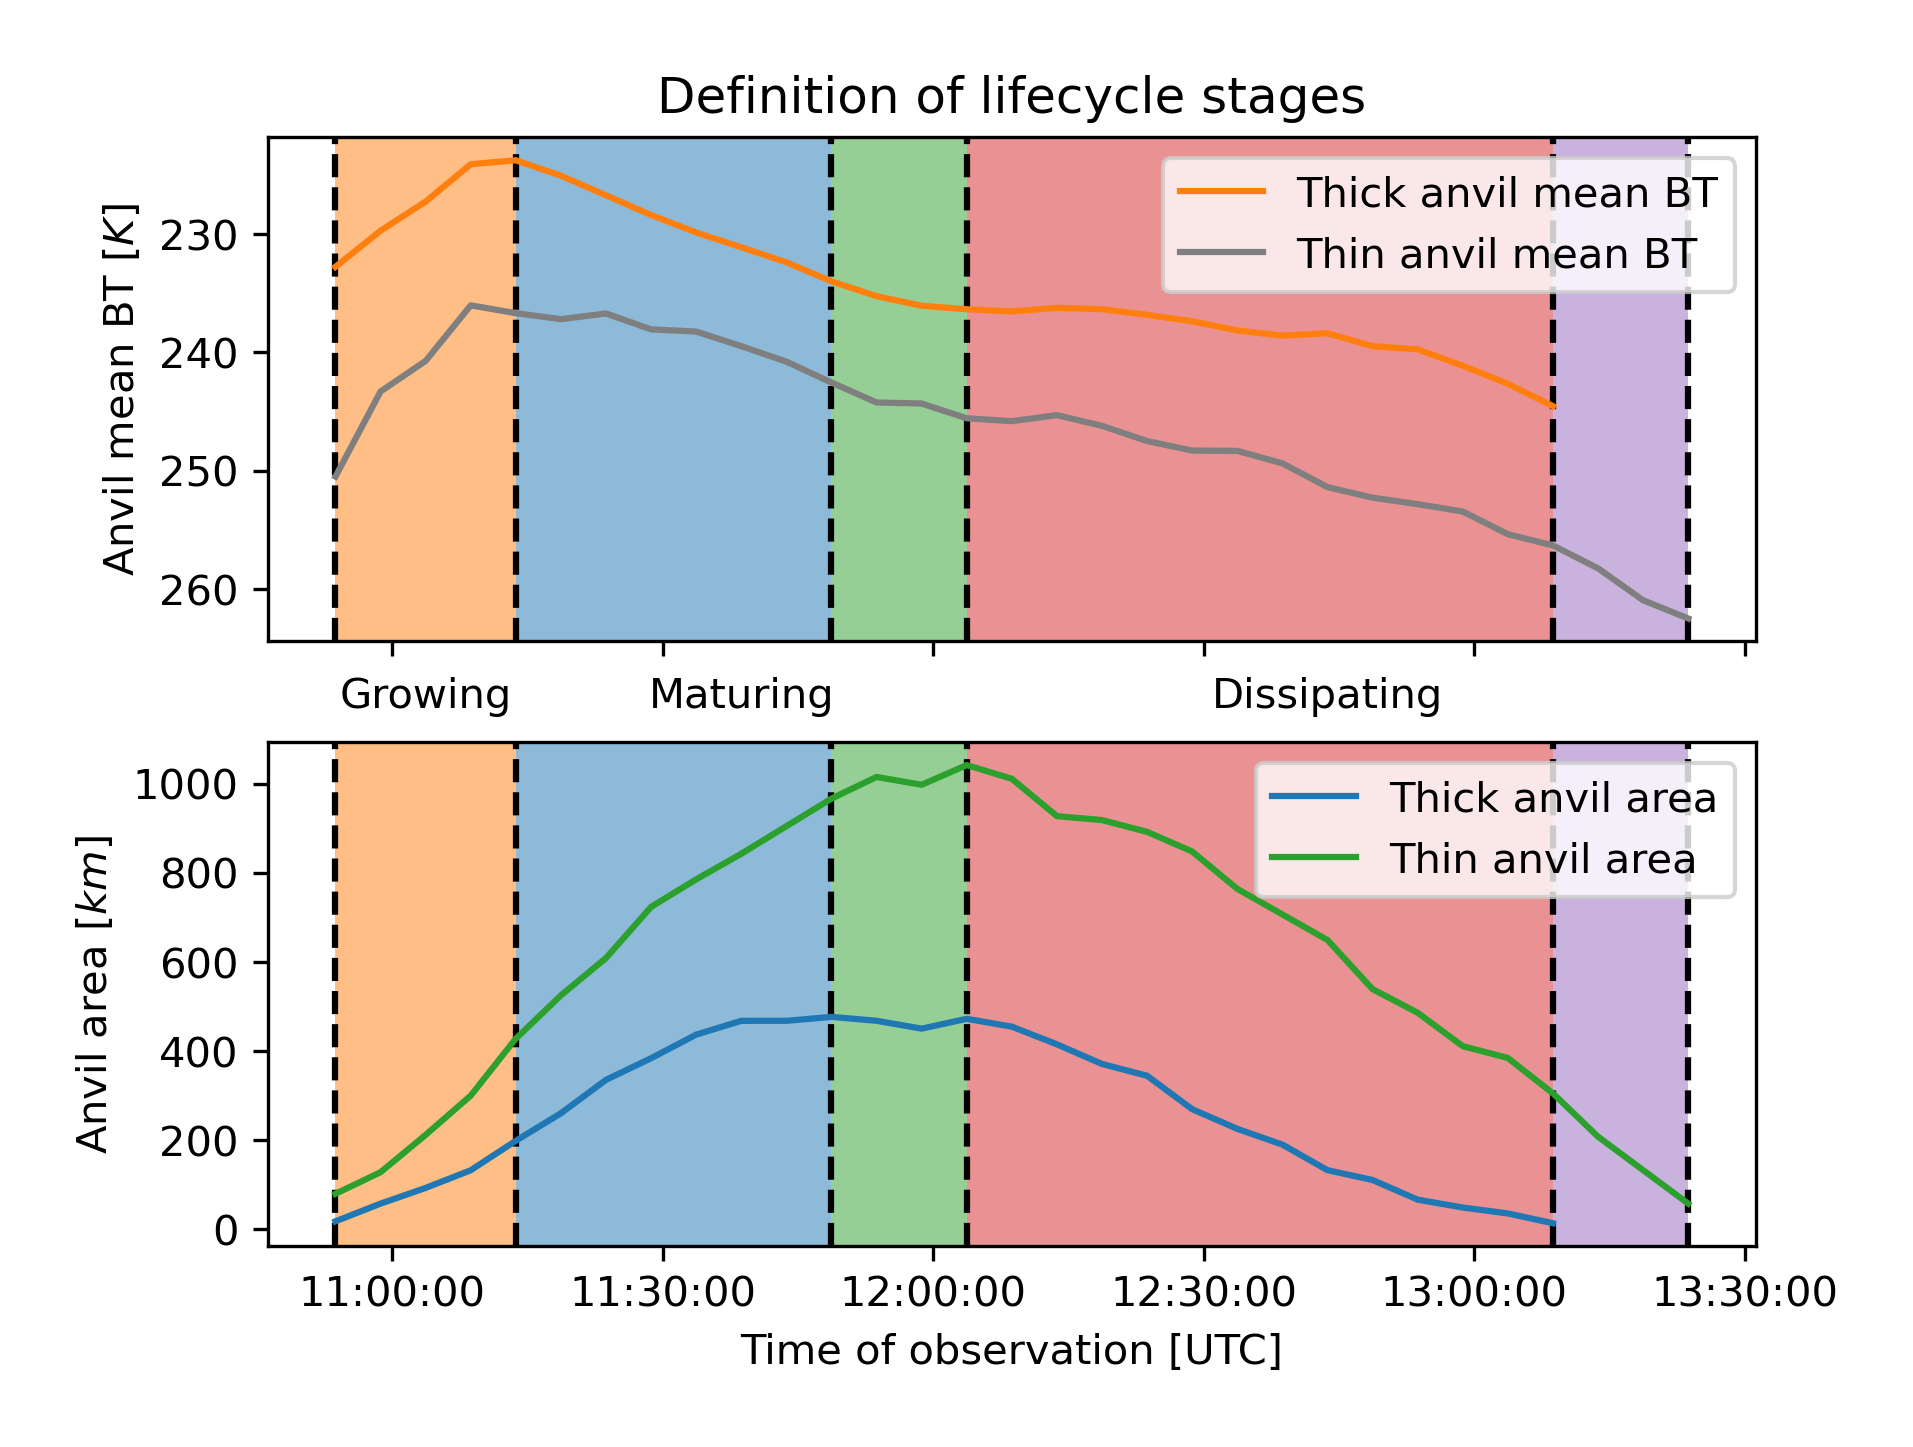
\includegraphics[width=\textwidth]{figures/chapter3_02.png}
    \caption[
    Definition of anvil lifecycle stages based on the method of \citet{futyan_deep_2007}
    ]{
    Definition of anvil lifecycle stages based on the method of \citet{futyan_deep_2007}. The top panel shows the evolution of the mean \acrshort{bt} of the thick and thin anvil regions over the \acrshort{dcc} lifecycle, and the bottom panel shows the evolution of the anvil area. The growing phase (orange) is defined as the time between initial detection and the minimum observed \acrshort{bt}. The mature phase for the thick (blue) and thin (green) anvil is defined as the time between the minimum \acrshort{bt} and maximum thick and thin anvil area respectively. The dissipating phase for the thick (red) and thin (purple) anvils is defined as the time between the anvil maximum area and the final time of detection of the thick and thin anvil respectively.
    }
    \label{fig:lifecycle_example}
\end{figure}

To analyse changes in the lifecycle of \acrshort{dcc}s, their lifetime is categorised based on the method developed by \citet{futyan_deep_2007}.
This method separates the anvil cloud into growing, maturing and dissipating stages based on observations of \acrshort{bt} and anvil area.
\citeauthor{futyan_deep_2007}'s method defines the end of the growing phase as the time at which the anvil reaches its minimum observed \acrshort{bt}, and the end of the mature phase as the time at which the anvil reaches the maximum observed area.
While simple, this approach applies to a wide range of observed \acrshort{dcc}s including both isolated and organised convection.
Furthermore, by determining the anvil lifecycle only in terms of the observed anvil properties, the properties of the detected cores can be treated as independent variables allowing straightforward analysis of their impacts on \acrshort{dcc} lifecycle.

\citeauthor{futyan_deep_2007}'s method is extended in this chapter through consideration of the development of both thick and thin anvil, which results in the lifecycle stages shown in fig.~\ref{fig:lifecycle_example}.
The growing stage (orange) is defined as the time from the initial detection of the \acrshort{dcc} to the time at which the thick anvil has its coldest average \acrshort{bt}.
The thick anvil maturation stage (blue) occurs between this time and the time at which the thick anvil reaches its maximum area, and the thin anvil maturing stage (green) occurs until the thin anvil reaches its maximum area.
In this stage, the thin anvil continues to expand while the thick anvil begins to shrink.
The thick anvil dissipating stage (red) ends at the final detection time of the thick anvil, while the thin anvil dissipating stage (purple) ends at the final detection time of the thin anvil, which is also the final detection time of the tracked \acrshort{dcc}.
By increasing the granularity of the lifecycle definition in this manner, the impact of convective processes on \acrshort{dcc} lifecycle and structure may also be investigated.

\subsection{Composite analysis} \label{sec:composite_definition}

To compare how the structure of tracked \acrshort{dcc} evolve over their lifecycle, the area of their cores, thick and thin anvils is interpolated over a normalised lifetime.
In this normalised lifetime, 0 is defined as the time of initial core detection, and 1 is the time of the final anvil detection.
By normalising their lifetimes in this manner, the change over time of \acrshort{dcc}s with different lifetimes can be composited and compared.


\begin{figure}[tp]
    \centering
    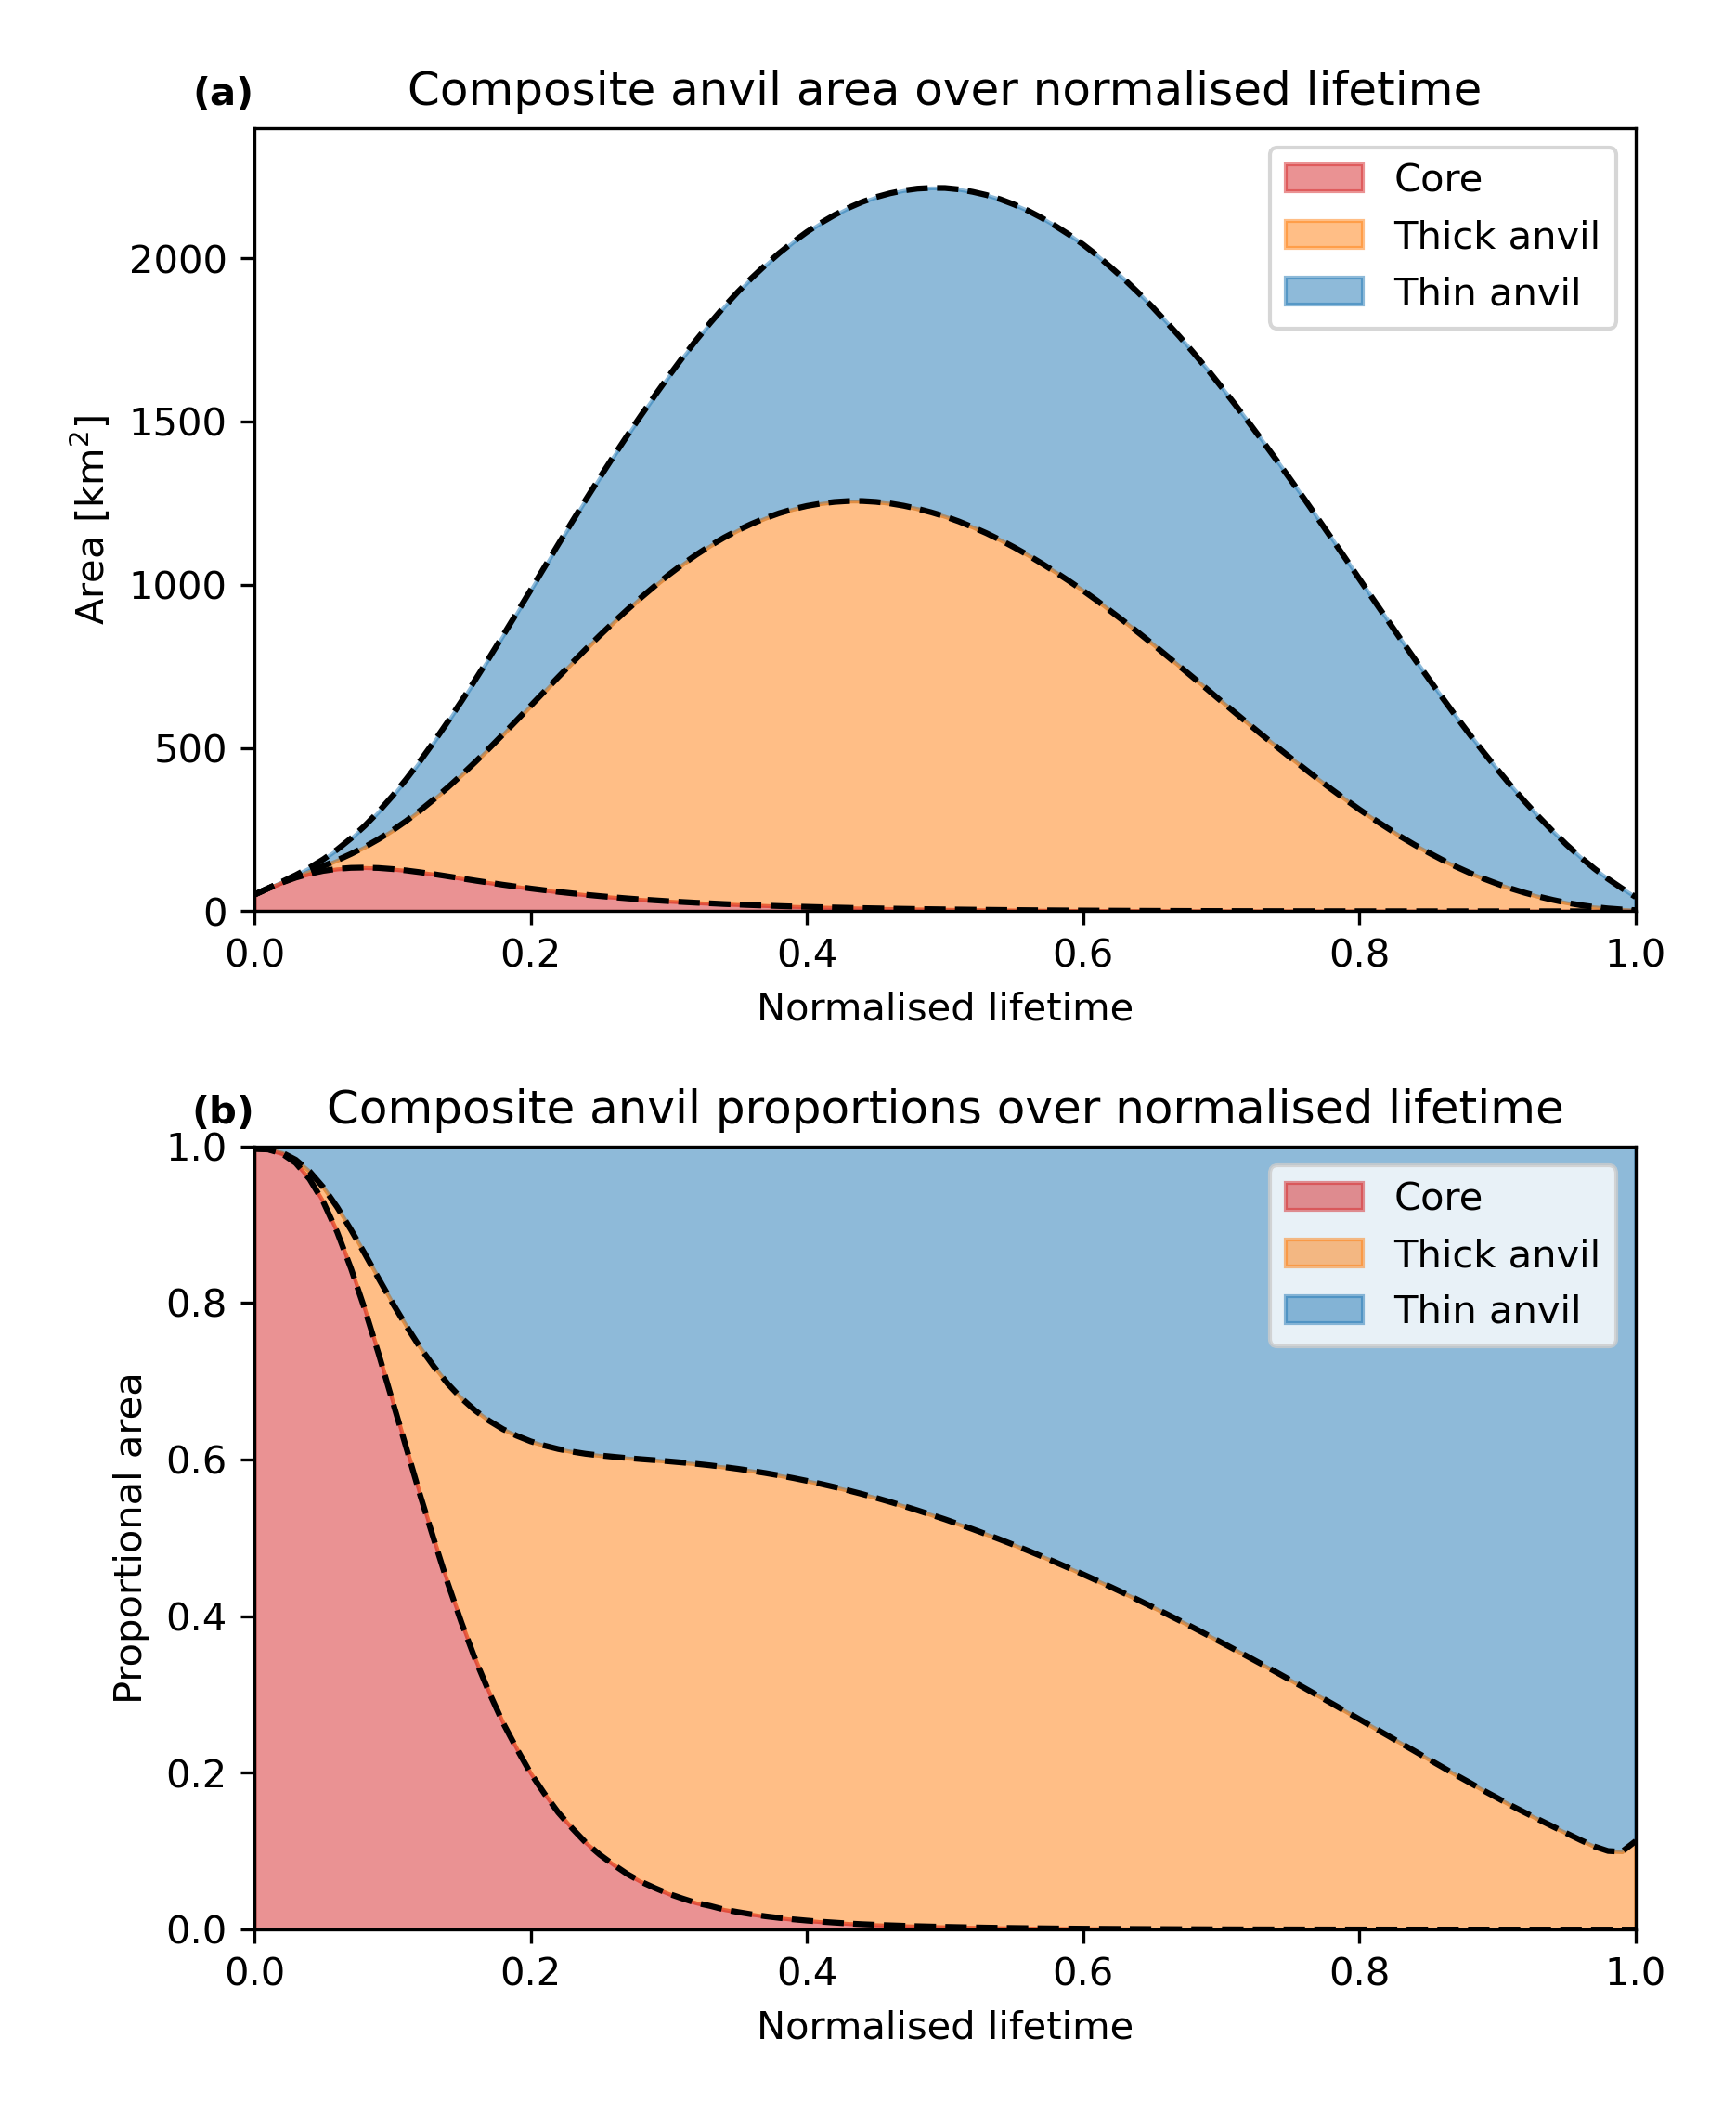
\includegraphics[width=\textwidth]{figures/chapter3_03.png}
    \caption[
    The average evolution of composites of cores (red), thick anvils (orange) and thin anvils (blue) over their normalised lifetimes
    ]{
    The average evolution of composites of cores (red), thick anvils (orange) and thin anvils (blue) over their normalised lifetimes, where 0 is the initial core detection time and 1 is the final anvil detection time. Panel (a) shows the average area of anvils, and (b) shows the proportion of the total area corresponding to each part of the anvil structure.
    }
    \label{fig:composite_example}
\end{figure}

An example composite of the average properties of all analysed anvils in this chapter is shown in fig.~\ref{fig:composite_example}.
Figure~\ref{fig:composite_example}\,a shows the average change in area of the core (red), thick anvil (orange) and thin anvil (blue) over the normalised lifetime of the \acrshort{dcc}s.
Figure~\ref{fig:composite_example}\,b shows how these areas change as a proportion of the net \acrshort{dcc} area.
This shows how, on average, the structure of \acrshort{dcc}s evolves over their lifetime.
Initially, the \acrshort{dcc} consists entirely of a growing core, with the initial anvil formation occurring between 10\% and 20\% of the \acrshort{dcc} lifetime.
The initial expansion of the anvil is mostly thin, likely because the majority of the mass flux is still travelling upwards, and the area of thick anvil is covered by the developing core.
Between 20\% and 40\% of the normalised lifetime, while the anvil is maturing, the thick and thin anvil expand at similar rates and so the proportion of thin anvil remains consistent.
Beyond this point, the thick anvil reaches its maximum area before the thin anvil and dissipates faster, and the fraction of the thin anvil increases until the end of the \acrshort{dcc} lifecycle.
Note that the average thin anvil fraction does not reach 100\% at the end of the normalised lifetime due to the presence of some \acrshort{dcc}s where the dissipation of the thick and thin anvil are recorded at the same time.

Through the use of composite analysis, the change in anvil structure throughout the \acrshort{dcc} lifecycle can be investigated. 
This allows the study of responses to prior observed convective processes, rather than limiting our analysis to bulk properties or snapshots.

\section{Results}

\subsection{Change in thin anvil fraction with intensity and organisation}

%f
\begin{figure}[tp]
    \centering
    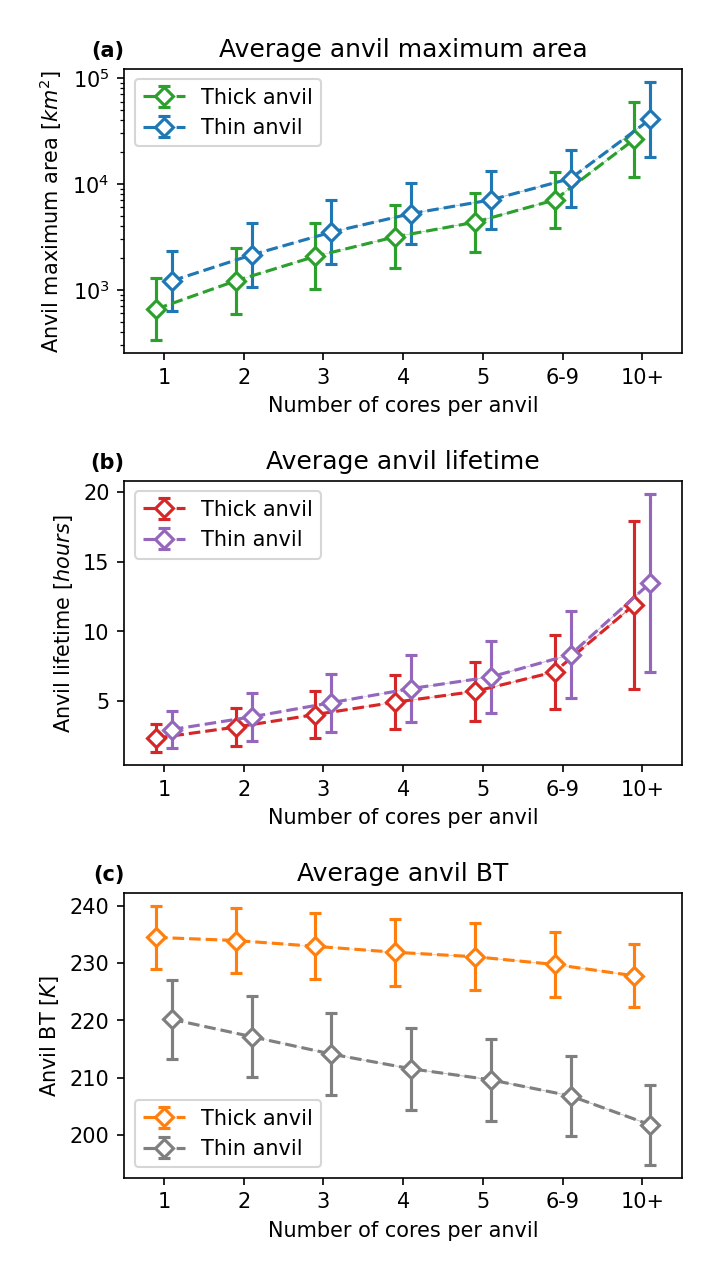
\includegraphics[width=0.75\textwidth]{figures/chapter3_04.png}
    \caption[
    Thin anvil proportion of anvils categorised by mean anvil \acrshort{bt}, initial core cooling rate and number of cores
    ]{
    Thin anvil proportion of anvils categorised by (a) mean anvil \acrshort{bt}, (b) initial core cooling rate, and (c) number of cores. Black error bars show the standard error of the mean, and coloured error bars show the standard deviation.
    }
    \label{fig:thin_anvil_proportion}
\end{figure}

%f
\begin{figure}[tp]
    \centering
    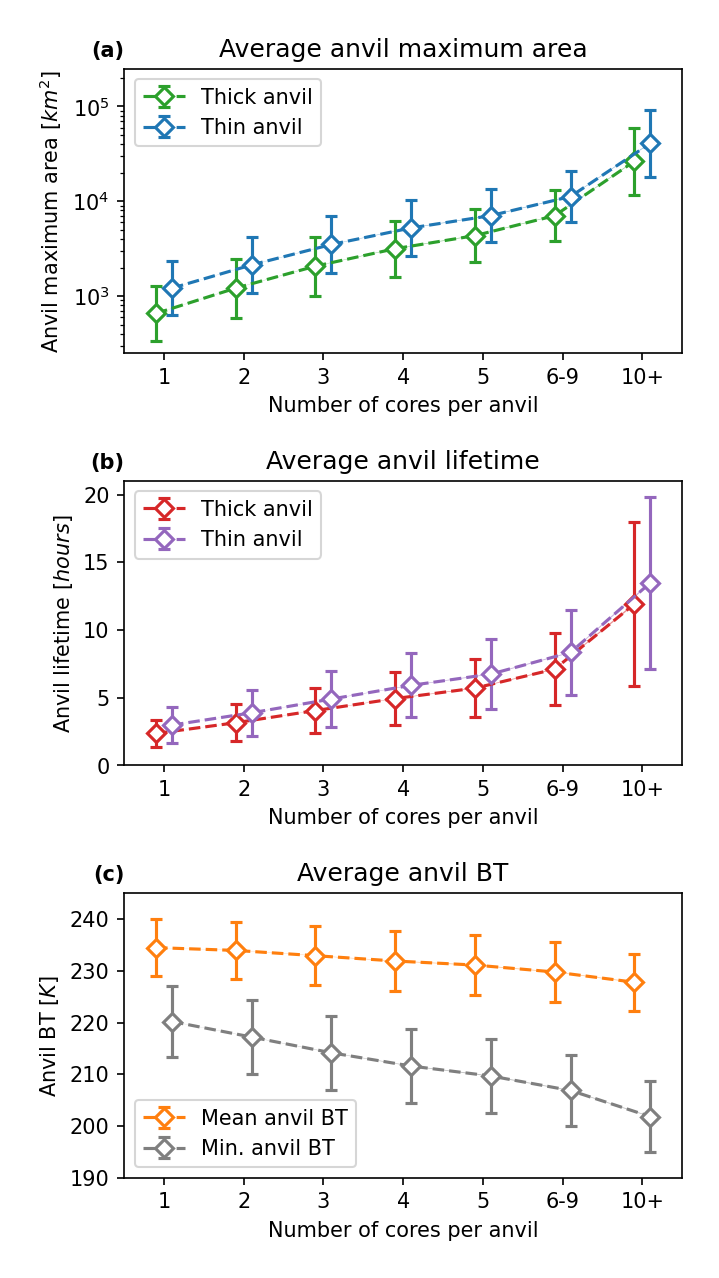
\includegraphics[width=0.75\textwidth]{figures/chapter3_05.png}
    \caption[
    A comparison of the change in thin anvil proportion with maximum core cooling rate and number of cores for four different regions
    ]{
    A comparison of the change in thin anvil proportion with (a) maximum core cooling rate and (b) number of cores for four different regions: sea (blue diamond markers), land (orange square markers), tropics (\textless 30\,\textdegree N; red downward triangle markers) and mid-latitudes (\textgreater 30\,\textdegree N; purple upward triangle markers). Error bars show the standard deviation of the thin anvil fraction.
    }
    \label{fig:regional_thin_anvil_proportion}
\end{figure}

To begin, the net thin anvil fraction of observed anvils is compared with the mean anvil \acrshort{bt}, initial core maximum cooling rate and number of cores.
Figure~\ref{fig:thin_anvil_proportion}\,a shows how the thin anvil proportion changes with the average thick anvil \acrshort{bt}.
Note that only the thick anvil \acrshort{bt} is considered to avoid a dependence between the anvil \acrshort{bt} and the thin anvil area.
There is an increase of thin anvil proportion with the average anvil \acrshort{bt}, agreeing with the results of \citet{protopapadaki_upper_2017}.
Figure~\ref{fig:thin_anvil_proportion}\,b compares how the thin anvil fraction changes with the maximum cooling rate of the initial core associated with the anvil, and again shows a positive relation between the strength of convection and the thin anvil fraction.
While the value of the thin anvil fraction differs from that observed in previous studies, this is expected as both studies use different methods to define thick and thin.
In addition, in this chapter, the proportion is measured over the entire \acrshort{dcc} lifetime rather than at a single point in time.

In fig.~\ref{fig:thin_anvil_proportion}\,c, the thin anvil fraction is compared to the number of cores associated with each anvil.
In contrast to fig.~\ref{fig:thin_anvil_proportion}\,b and c, there is a decrease in the thin anvil fraction with an increase in the number of cores.
As this occurs despite the tendency for multiple-core anvils to have colder average \acrshort{bt}, this indicates that further factors are involved in the thin anvil fraction than the temperature and height of the anvil.

To ensure that these relationships are not caused by differences in the properties and distributions of \acrshort{dcc}s across different regions, the relationship between cooling rate and number of cores and the thin anvil fraction is further separated into four different regions, shown in fig.~\ref{fig:regional_thin_anvil_proportion}.
As with previous studies, the fraction of thin anvil is very similar for \acrshort{dcc}s observed over land and ocean.
While there is a difference in the thin anvil fraction of approximately 0.05 between \acrshort{dcc}s located in the tropics and mid-latitudes (defined as \textless 30\,\textdegree N and \textgreater 30\,\textdegree N respectively), this difference decreases with increasing convective intensity.
Overall, the near identical relationship of thin anvil fraction to intensity and organisation across multiple regions indicates that this is linked to the convective processes themselves, rather than a co-variance with local conditions.

\subsection{Impact of intensity and organisation on \acrshort{dcc} properties}

Both the intensity and organisation of \acrshort{dcc} cores have impacts on the properties of their anvil clouds.
This section will investigate how these processes affect the bulk properties of these anvils; the anvil maximum area and the anvil lifetime for both thick and thin anvils, and the anvil \acrshort{bt}.
While comparing the bulk properties of these anvils provides an indication of how their structure changes, it does not fully explain the differences shown in figs.~\ref{fig:thin_anvil_proportion} and \ref{fig:regional_thin_anvil_proportion}.

%f
\begin{figure}[tp]
    \centering
    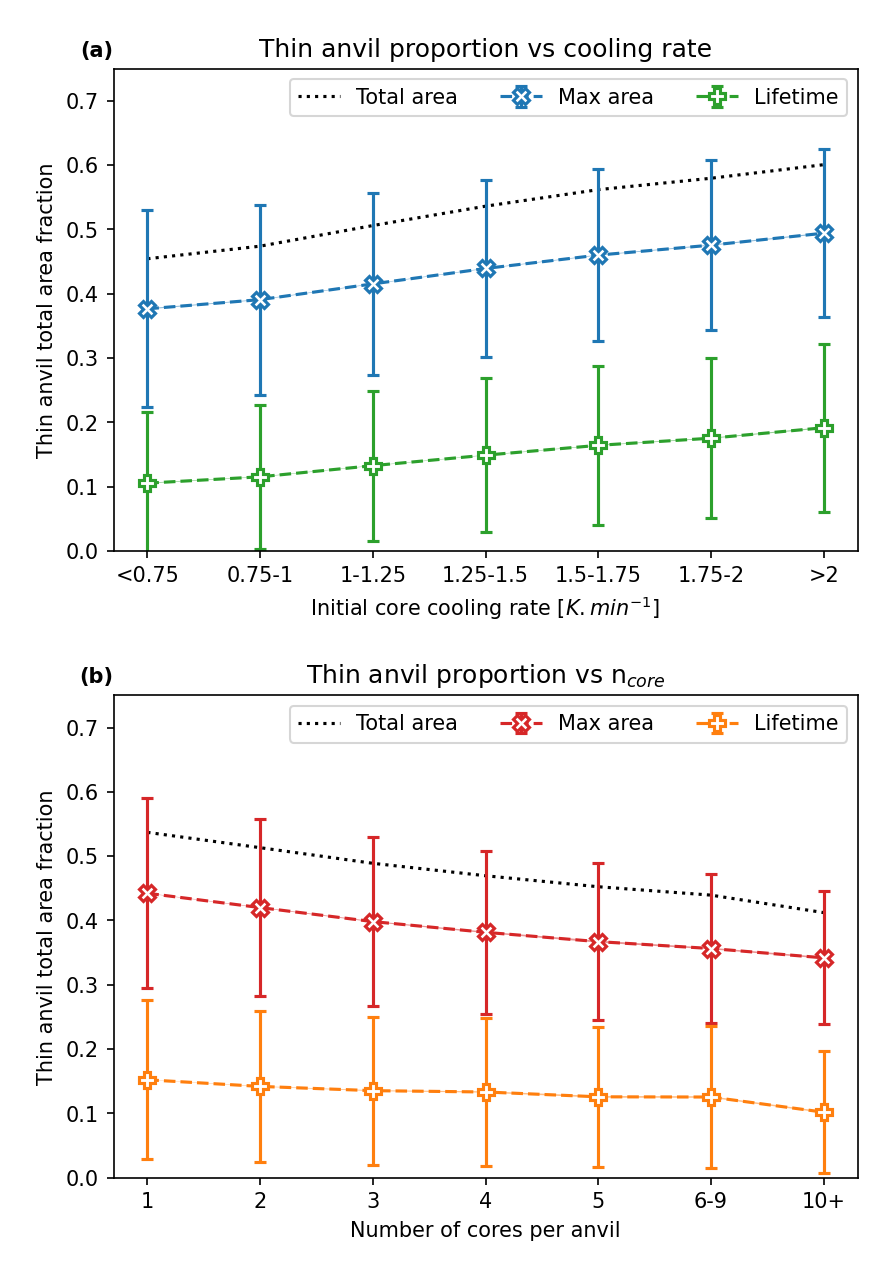
\includegraphics[width=0.75\textwidth]{figures/chapter3_06.png}
    \caption[
    The effect of initial core cooling rate on maximum anvil area, anvil lifetime, and mean and minimum \acrshort{bt}
    ]{
    The effect of initial core cooling rate on (a) maximum anvil area, (b) anvil lifetime, and (c) mean and minimum \acrshort{bt}. Error bars show the standard deviation. Points have been staggered to show the thick and thin anvil properties more clearly, but correspond to the same tick marks on the x axis.
    }
    \label{fig:anvil_cooling_rate_properties}
\end{figure}

Figure~\ref{fig:anvil_cooling_rate_properties} shows how the area, lifetime and \acrshort{bt} of \acrshort{dcc}s change with the core cooling rate.
Figure~\ref{fig:anvil_cooling_rate_properties}\,a shows that the average thick and thin anvil maximum areas vary very little with cooling rate, except for at the highest observed values of cooling rate.
There is however a slight widening in the gap between the thick and thin anvil maximum areas with increasing core cooling rate, as the thin anvil increases in maximum area while the thick anvil remains consistent.
Figure~\ref{fig:anvil_cooling_rate_properties}\,b shows that while the average thick anvil lifetime remains constant with increasing core cooling rate, the thin anvil lifetime increases.
There is also a consistent decrease in both average and minimum thick anvil \acrshort{bt} with cooling rate, shown in fig.~\ref{fig:anvil_cooling_rate_properties}\,c.
This change in anvil \acrshort{bt} with the core intensity agrees with the results shown previously in fig.~\ref{fig:core_cooling_rate_relations}\,b which showed that more intense cores have colder minimum \acrshort{bt}.

%f
\begin{figure}[tp]
    \centering
    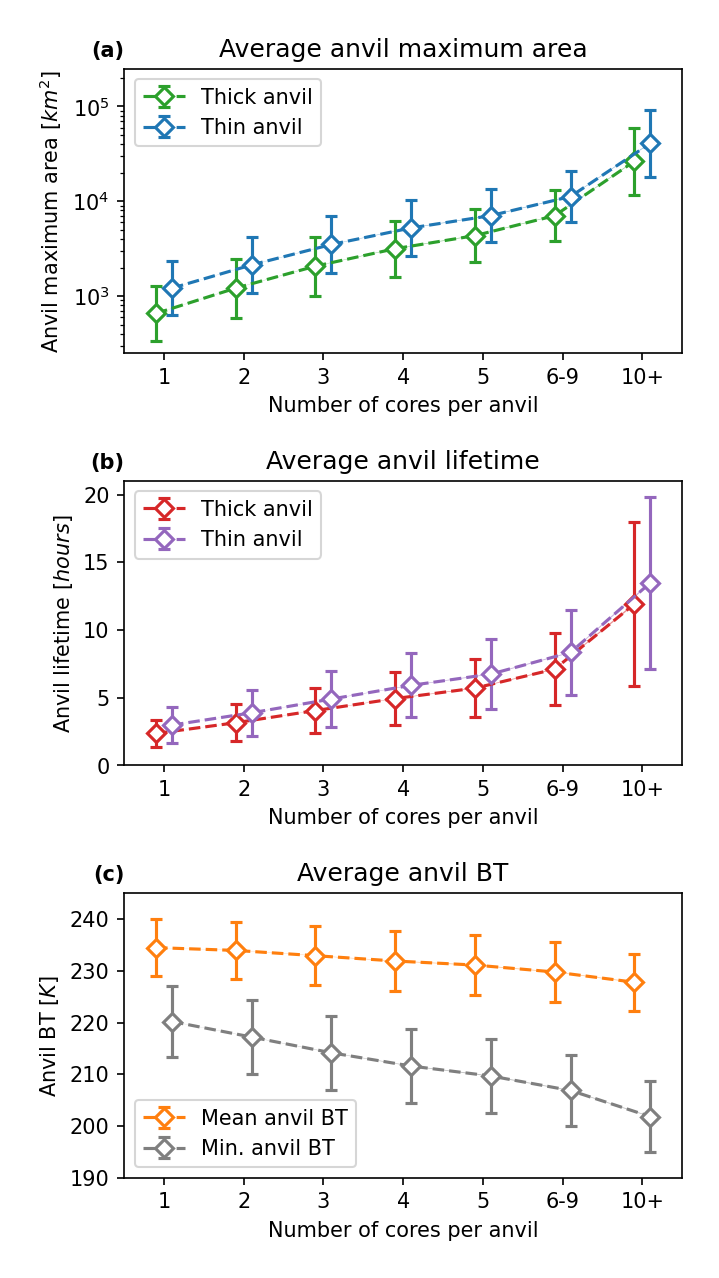
\includegraphics[width=0.75\textwidth]{figures/chapter3_07.png}
    \caption[
    The effect of the number of cores on maximum anvil area, anvil lifetime, and mean and minimum \acrshort{bt}
    ]{
    The effect of the number of cores on (a) maximum anvil area, (b) anvil lifetime, and (c) mean and minimum \acrshort{bt}. Error bars show the standard deviation. Points have been staggered to show the thick and thin anvil properties more clearly, but correspond to the same tick marks on the x axis.
    }
    \label{fig:anvil_number_of_cores_properties}
\end{figure}

In fig.~\ref{fig:anvil_number_of_cores_properties} the change of anvil properties with the number of cores is considered.
Figure~\ref{fig:anvil_number_of_cores_properties}\,a shows that both the thick and thin anvil maximum area increase substantially with an increasing number of cores (note that it is plotted against a log scale).
However, the thin anvil area increases at a slower rate proportional to the thick anvil.
Similarly, there is an increase in both the thick and thin anvil lifetime with increasing number of cores shown in fig.~\ref{fig:anvil_number_of_cores_properties}\,b.
There is a similar rate of the decrease of average anvil \acrshort{bt} with the number of cores in fig.~\ref{fig:anvil_number_of_cores_properties}\,c as shown in relation to core cooling rate in fig.~\ref{fig:anvil_cooling_rate_properties}\,c.
The minimum anvil \acrshort{bt} decreases at a notably faster rate with the increasing number of cores, however.
Although this is indicative of an increased likelihood of overshooting cores in more organised \acrshort{dcc}s, it must also be noted that the larger area of these systems also makes it more likely to observe a colder minimum pixel value.

%f
\begin{figure}[tp]
    \centering
    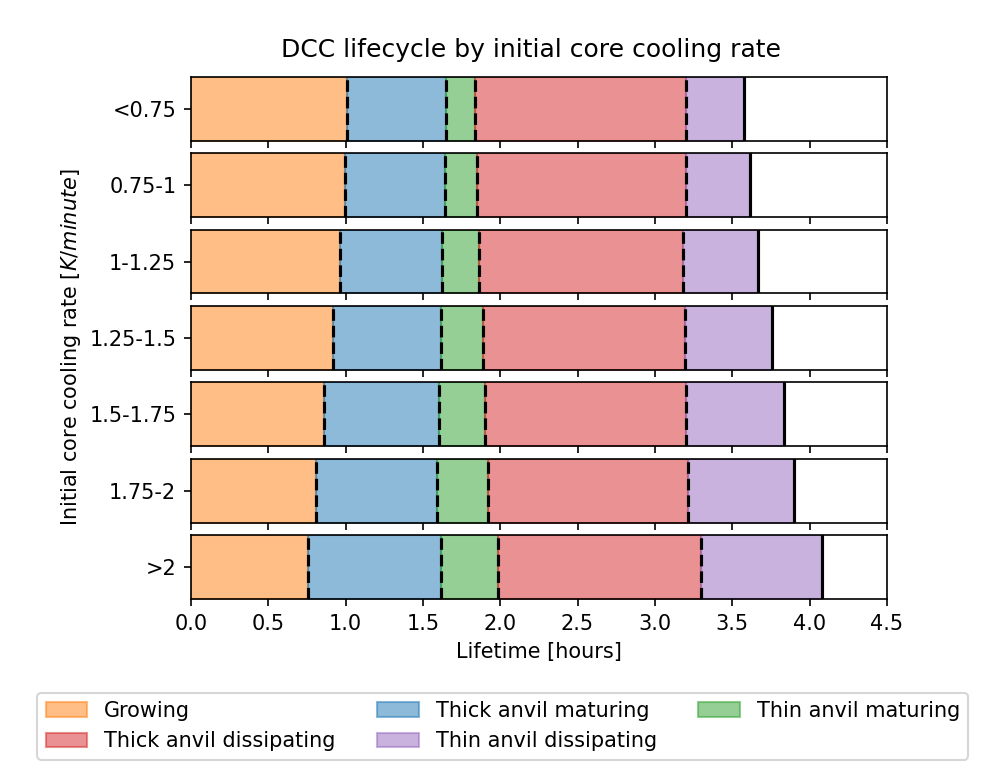
\includegraphics[width=0.75\textwidth]{figures/chapter3_08.png}
    \caption[
    A comparison of the proportion of thin anvil measured at the time of maximum anvil area, and the proportional difference in lifetime, compared to the overall thin anvil proportion.
    ]{
    A comparison of the proportion of thin anvil measured at the time of maximum anvil area, and the proportional difference in lifetime, compared to the overall thin anvil proportion. Panel (a) shows the change in thin anvil proportion with core cooling rate, and (b) shows the changes with the number of cores. In both panels, the black dotted line shows the total thin anvil proportion over the entire \acrshort{dcc} lifecycle. Error bars show the standard deviation of the thin anvil fraction, and while some extend below zero all measured thin anvil fractions are positive.
    }
    \label{fig:max_area_and_lifetime_contributions}
\end{figure}

The changes in anvil properties with intensity and convection are intriguing due to both their differences and similarities.
Both processes result in anvils with colder \acrshort{bt}, which is commonly used as a proxy for convective intensity.
However, the differences in the changes in anvil areas and lifetimes show that these processes cannot be lumped together so simply.


In fig.~\ref{fig:max_area_and_lifetime_contributions}, the proportion of observed thin anvil fraction that can be attributed to the bulk changes in anvil maximum area and lifetime is shown.
The proportional difference in the maximum area of the thick and thin anvils represents approximately 80\% of the change in thin anvil fraction across both convective intensity and organisation.
This shows that while the trend in thin anvil fraction can be captured by snapshot observations from polar-orbiting satellites, they will underestimate the total thin anvil fraction over the entire \acrshort{dcc} lifetime.
The proportional difference in the thick and thin anvil lifetimes shows a smaller contribution to the net thin anvil fraction.
Furthermore, there is a stronger (positive) trend of the lifetime proportion with intensity and a weaker (negative) trend with organisation.
Note that while some of the error bars (showing the standard deviation) extend below zero, all values for the thin anvil fraction are positive.


\subsection{Changes in \acrshort{dcc} lifecycle with intensity and organisation} \label{sec:lifecycle_results}

It is clear from the impact on anvil lifetime that both the intensity and organisation of convection affect \acrshort{dcc} lifecycle.
Furthermore, fig.~\ref{fig:max_area_and_lifetime_contributions} shows that these different processes have different impacts on the lifecycle that warrant further investigation.
This section will focus on the effect of both convective intensity and organisation on the different lifecycle stages of \acrshort{dcc}s.
The modified \citeauthor{futyan_deep_2007} method explained in section~\ref{sec:lifecycle_definition} is used throughout to separate the anvil lifecycle into growing, mature and dissipating stages.

%f
\begin{figure}[tp]
    \centering
    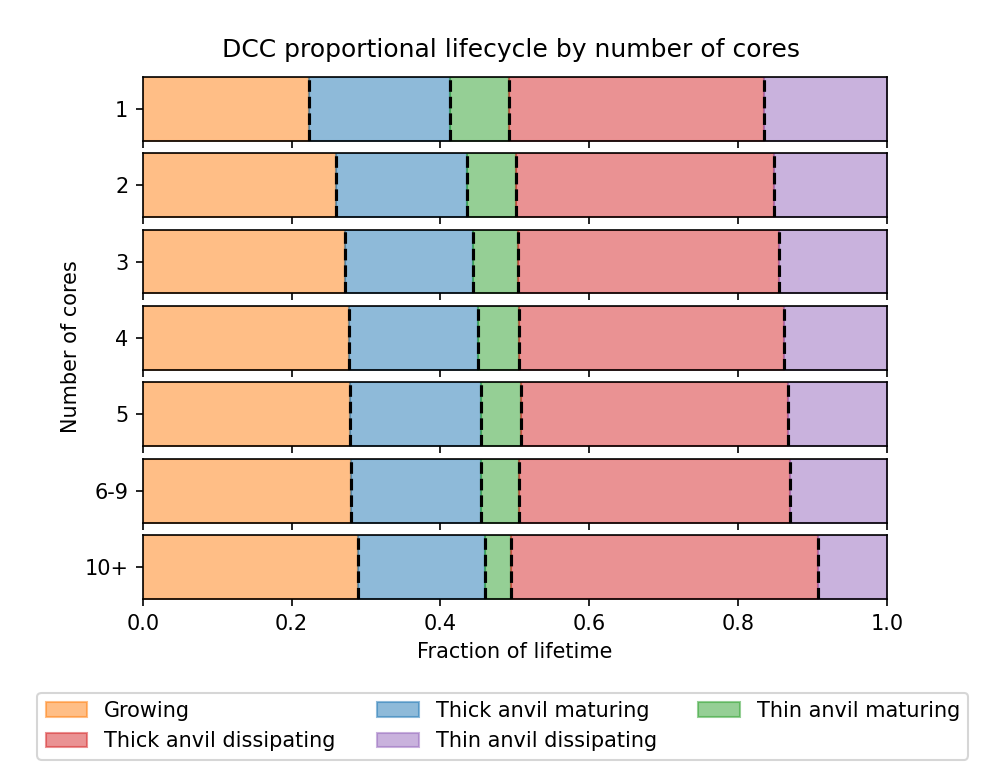
\includegraphics[width=\textwidth]{figures/chapter3_09.png}
    \caption[
    The average lifetime of each lifecycle stage for anvils categorised by their initial core cooling rate
    ]{
    The lifetime of each of the lifecycle stages, as defined in section~\ref{sec:lifecycle_definition}, for anvils categorised by their initial core cooling rate.
    }
    \label{fig:anvil_cooling_rate_absolute_lifecycle}
\end{figure}

Figure~\ref{fig:anvil_cooling_rate_absolute_lifecycle} shows the lifetime of the different lifecycle stages for \acrshort{dcc}s with increasing core cooling rates.
The lifetime of the growing stage decreases from 1 hour to 45 minutes for the most intense convection.
While these growing lifetimes are longer than those of the detected cores shown in fig.~\ref{fig:core_cooling_rate_relations}, the trend agrees with the shorter lifetime for more intense cores.
Despite the colder \acrshort{bt} and hence higher cloud top heights exhibited by these \acrshort{dcc}s, the stronger vertical growth rates result in an anvil which reaches its minimum \acrshort{bt} in a shorter time frame.

The timing of the maximum extent of the thick anvil remains consistent at just over 1.5 hours for all cooling rates, while the time of the maximum thin anvil area increases from 1 hour 45 minutes to 2 hours for the most intense \acrshort{dcc}s.
Similarly, the timing of the dissipation of the thick remains consistent at just over 3 hours for most cooling rates, while the thin anvil dissipation time increases from 3.5 hours to 4 hours for more intense \acrshort{dcc}s.
These findings reinforce what was shown in fig.~\ref{fig:anvil_cooling_rate_properties}, that the core cooling rate affects the lifetime of the thin anvil but not the thick anvil.

%f
\begin{figure}[tp]
    \centering
    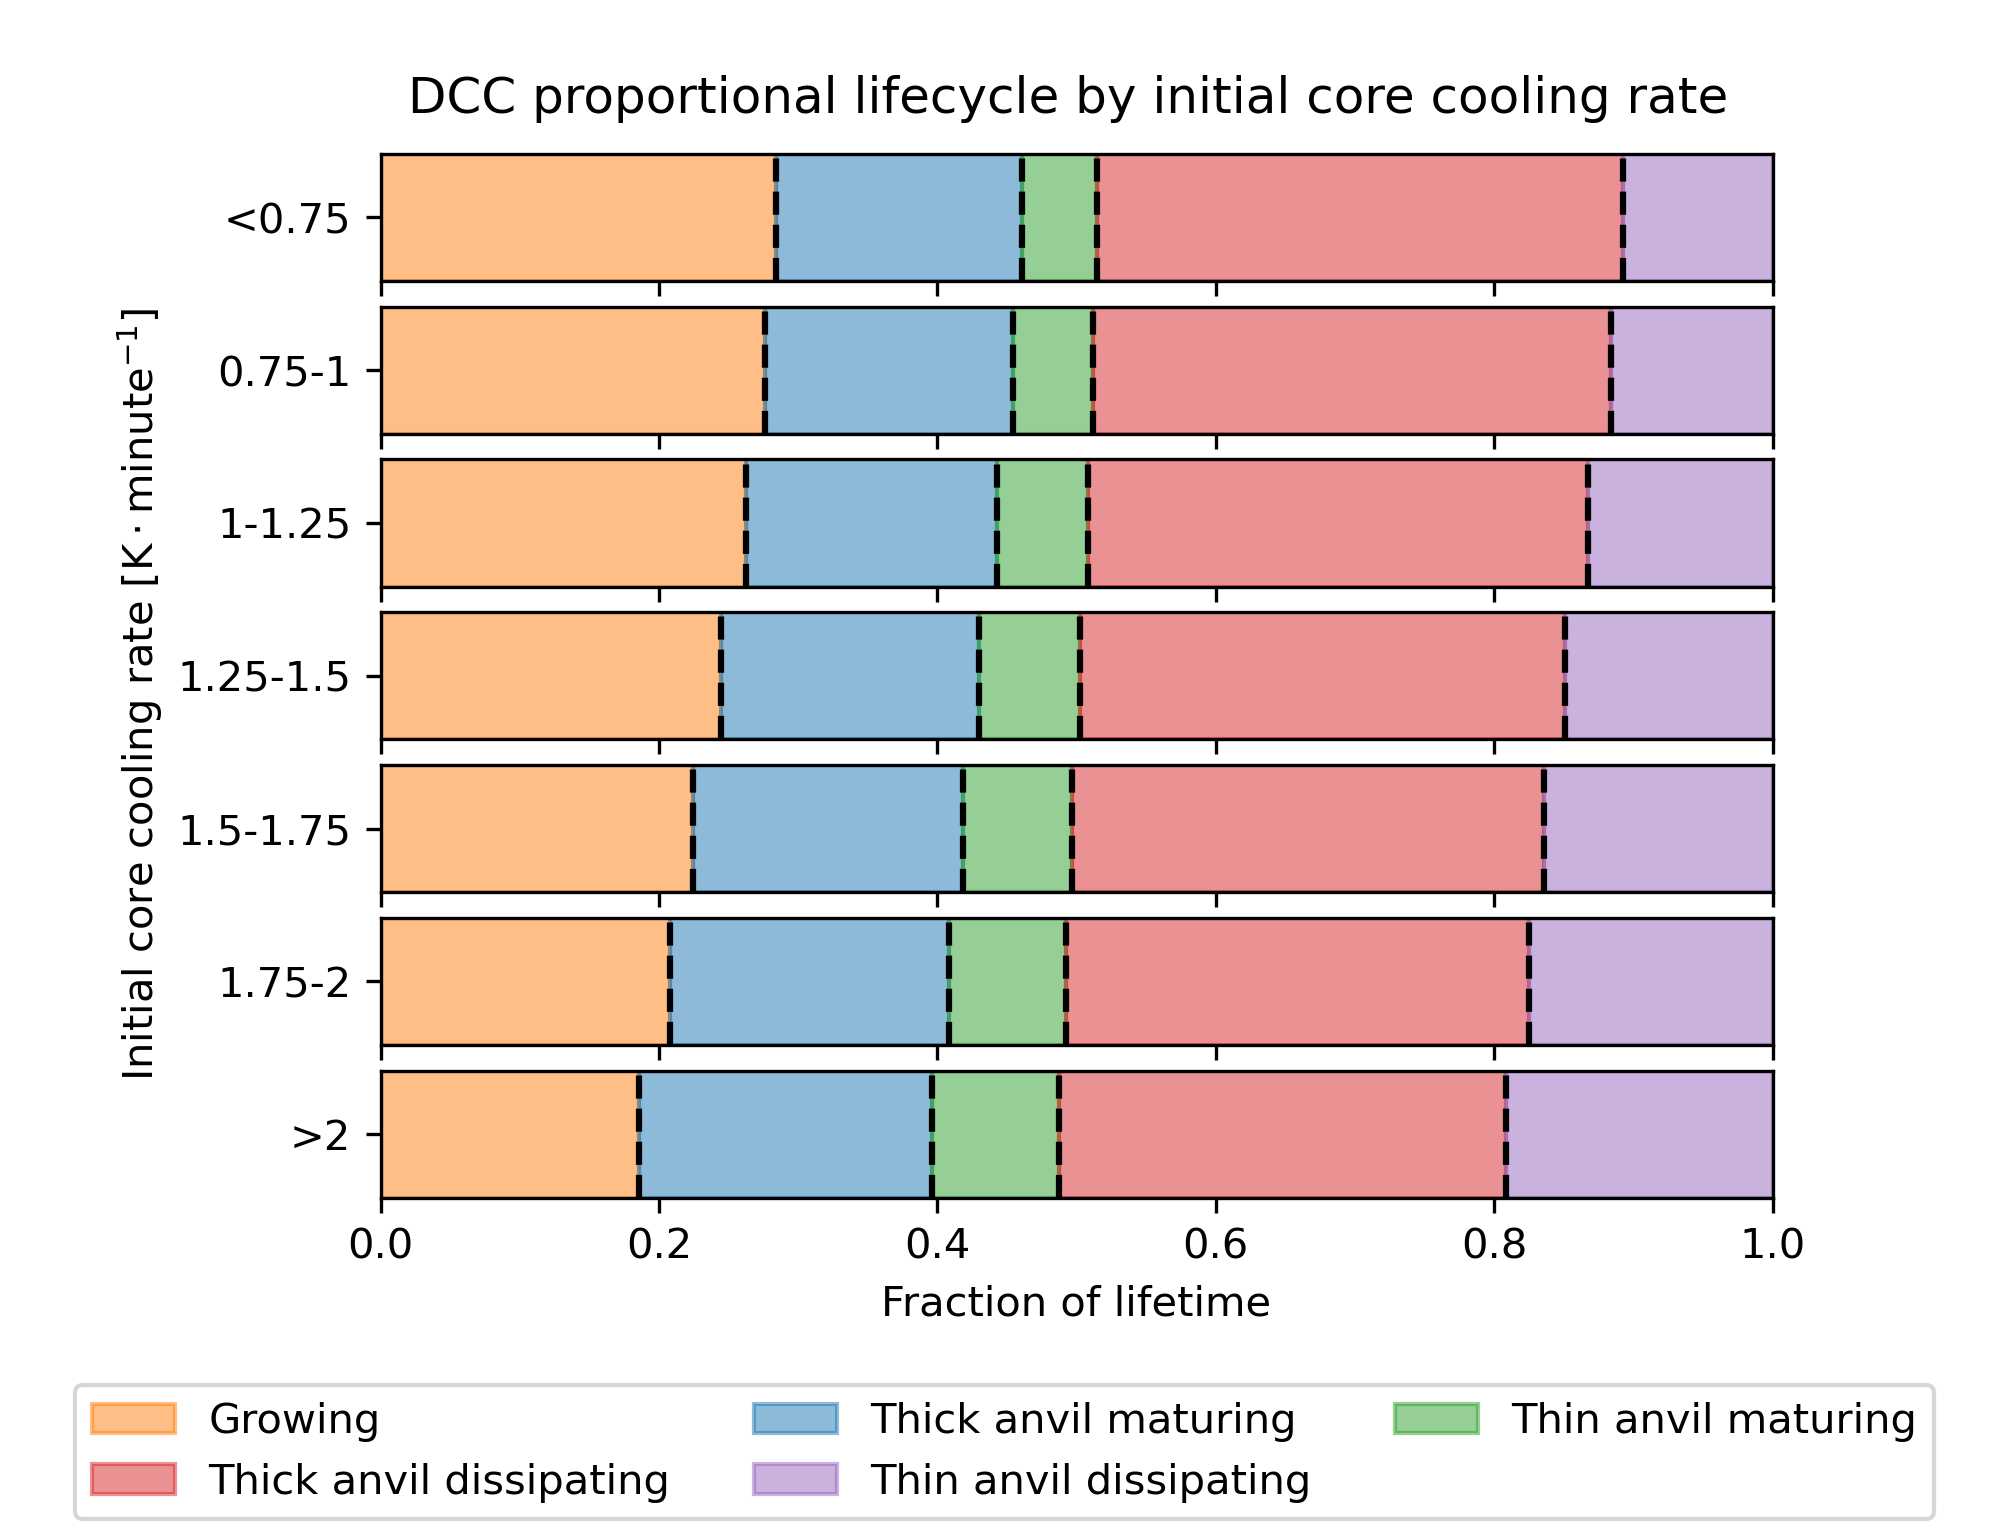
\includegraphics[width=\textwidth]{figures/chapter3_10.png}
    \caption[
    The average fraction of anvil lifetime of each lifecycle stage for anvils categorised by initial core cooling rate
    ]{
    The average fraction of anvil lifetime of each of the lifecycle stages defined in section~\ref{sec:lifecycle_definition} for anvils categorised by initial core cooling rate. Each bar is normalised such that the total length of the row is equal to the mean thin anvil lifetime of its cooling rate bin.
    }
    \label{fig:anvil_cooling_rate_proportional_lifecycle}
\end{figure}

Figure~\ref{fig:anvil_cooling_rate_proportional_lifecycle} displays the average proportion of anvil lifetime spent in each of the stages shown in fig.~\ref{fig:anvil_cooling_rate_absolute_lifecycle}.
The anvil lifetime is normalised using the method described in section~\ref{sec:composite_definition}, where 0 is the time of the initial detection of the \acrshort{dcc} and 1 is the time of the final detection of the dissipating thin anvil.
By analysing these lifecycle stages as a proportion of the total lifetime, better insight is gained into how changes in lifecycle impact the structure and bulk properties of observed \acrshort{dcc}s.

The reduction in the lifetime of the growing phase and increase for thin anvil dissipation for more intense \acrshort{dcc}s is again apparent.
The time between these two stages, representing the period in which the thick anvil matures and then dissipates, lasts for around 60\% of the total anvil lifecycle for all core cooling rates.
The shorter growing period and longer thin anvil dissipating period act together to shift the evolution of the thick anvil earlier in the \acrshort{dcc} lifecycle for more intense \acrshort{dcc}s.
For \acrshort{dcc}s over land, where there is a pronounced peak in occurrence in the afternoon, it is expected that this shifts the time in which the anvil is at its thickest and has the largest extent earlier in the day, potentially increasing its \acrshort{sw} \acrshort{cre}.


%f
\begin{figure}[tp]
    \centering
    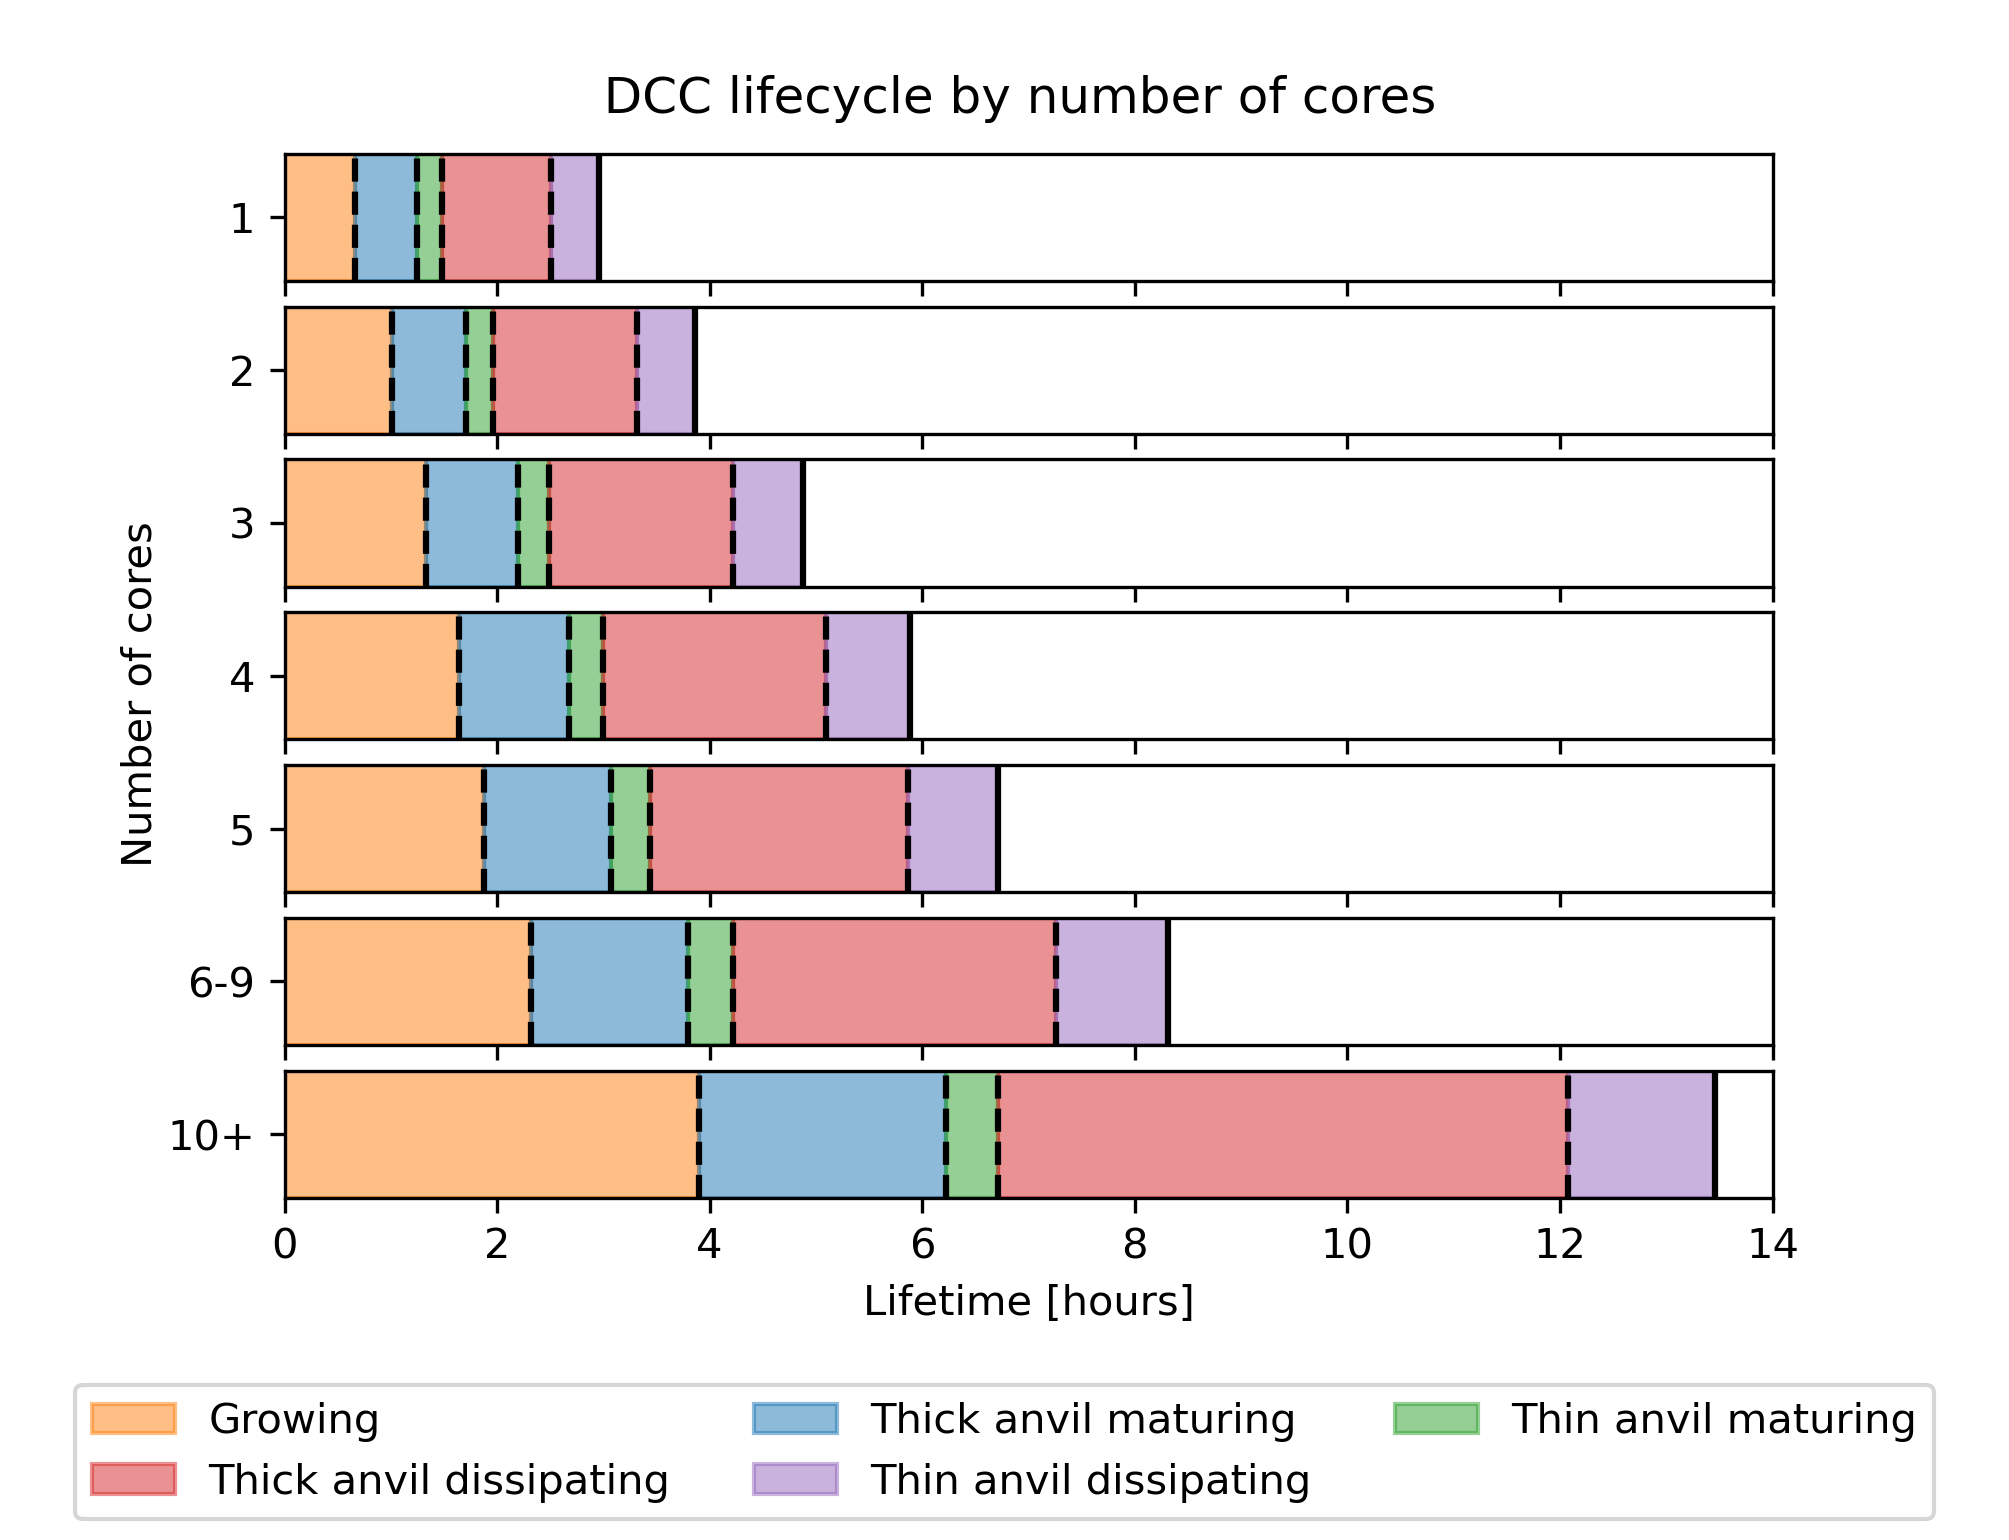
\includegraphics[width=\textwidth]{figures/chapter3_11.png}
    \caption[
    The average lifetime of each lifecycle stage for anvils categorised by number of cores
    ]{
    The average lifetime of each of the lifecycle stages defined in section~\ref{sec:lifecycle_definition} for anvils categorised by number of cores.
    }
    \label{fig:anvil_number_of_cores_absolute_lifecycle}
\end{figure}

Figure~\ref{fig:anvil_number_of_cores_absolute_lifecycle} shows how the timing of the different anvil stages changes with increasing number of cores.
It is immediately apparent that the large increase in overall lifetime with the number of cores shown in fig.~\ref{fig:anvil_number_of_cores_properties} also applies to each of the lifecycle stages.
This increase in lifetime occurs to such an extent that the average growing period for \acrshort{dcc}s with 10 or more cores lasts longer than the average of the entire lifetime of isolated \acrshort{dcc}s.
The large spread in lifetimes makes it difficult to compare how the lifecycle changes with organisation without normalising the lifetimes.

%f
\begin{figure}[tp]
    \centering
    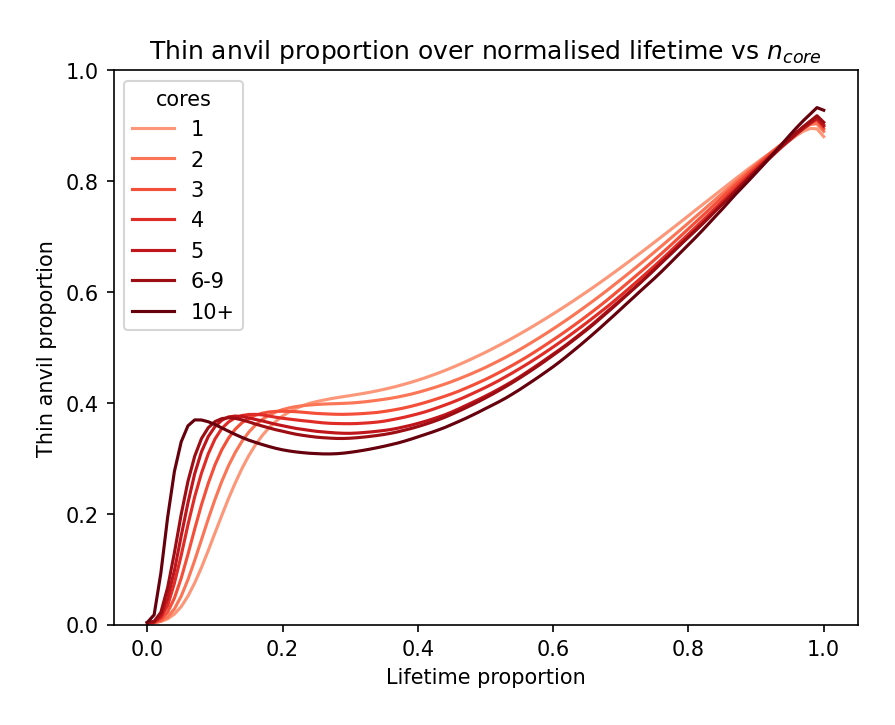
\includegraphics[width=\textwidth]{figures/chapter3_12.png}
    \caption[
    The average fraction of anvil lifetime of each lifecycle stage for anvils categorised by number of cores
    ]{
    The average fraction of anvil lifetime of each of the lifecycle stages defined in section~\ref{sec:lifecycle_definition} for anvils categorised by number of cores. Each bar is normalised such that the total length of the row is equal to the mean thin anvil lifetime of its number of cores bin.
    }
    \label{fig:anvil_number_of_cores_proportional_lifecycle}
\end{figure}

Figure~\ref{fig:anvil_number_of_cores_proportional_lifecycle} shows the lifetime of each lifecycle stage as a proportion of the total lifetime for \acrshort{dcc}s with different numbers of cores, in the same manner as used for fig.~\ref{fig:anvil_cooling_rate_proportional_lifecycle}.
In contrast to the effect of increasing intensity, with increasing organisation the length of the growing phase increases and the length of the thin anvil dissipating phase decreases as a proportion of the overall lifetime.
Similar behaviour is seen in the period from the start of the mature phase to the thick anvil dissipation, which remains a consistent length for all core counts.
With increasing organisation, this period shifts later in the lifetime of the \acrshort{dcc}.

It should be clarified, however, that these differences are only in relation to the proportion of total lifetime.
While more organised systems spend a smaller proportion of their lifetime in the thin anvil dissipating phase, the much greater overall lifetime means that this stage still lasts substantially longer than for \acrfull{dcc}s with fewer cores.


\subsection{Changes in thin anvil fraction over \acrshort{dcc} lifecycle} \label{sec:composite_results}

While the contrasting changes in \acrshort{dcc} lifecycle with increasing intensity and organisation (in particular the change in the thin anvil dissipating stage) go some way to explaining the difference in the thin anvil fraction, fig.~\ref{fig:max_area_and_lifetime_contributions} showed that the change in lifetime cannot account for the change in thin anvil fraction alone.
The contrasting changes in lifecycle do, however, indicate that the two convective processes influence how \acrshort{dcc}s evolve over their entire lifetimes.
To further investigate how convective processes impact structure and lifecycle, the composite area approach described in section~\ref{sec:composite_definition} is used to show how the thin anvil fraction evolves over the anvil lifecycle for \acrshort{dcc}s with differing core cooling rates and number of cores.


%f
\begin{figure}[tp]
    \centering
    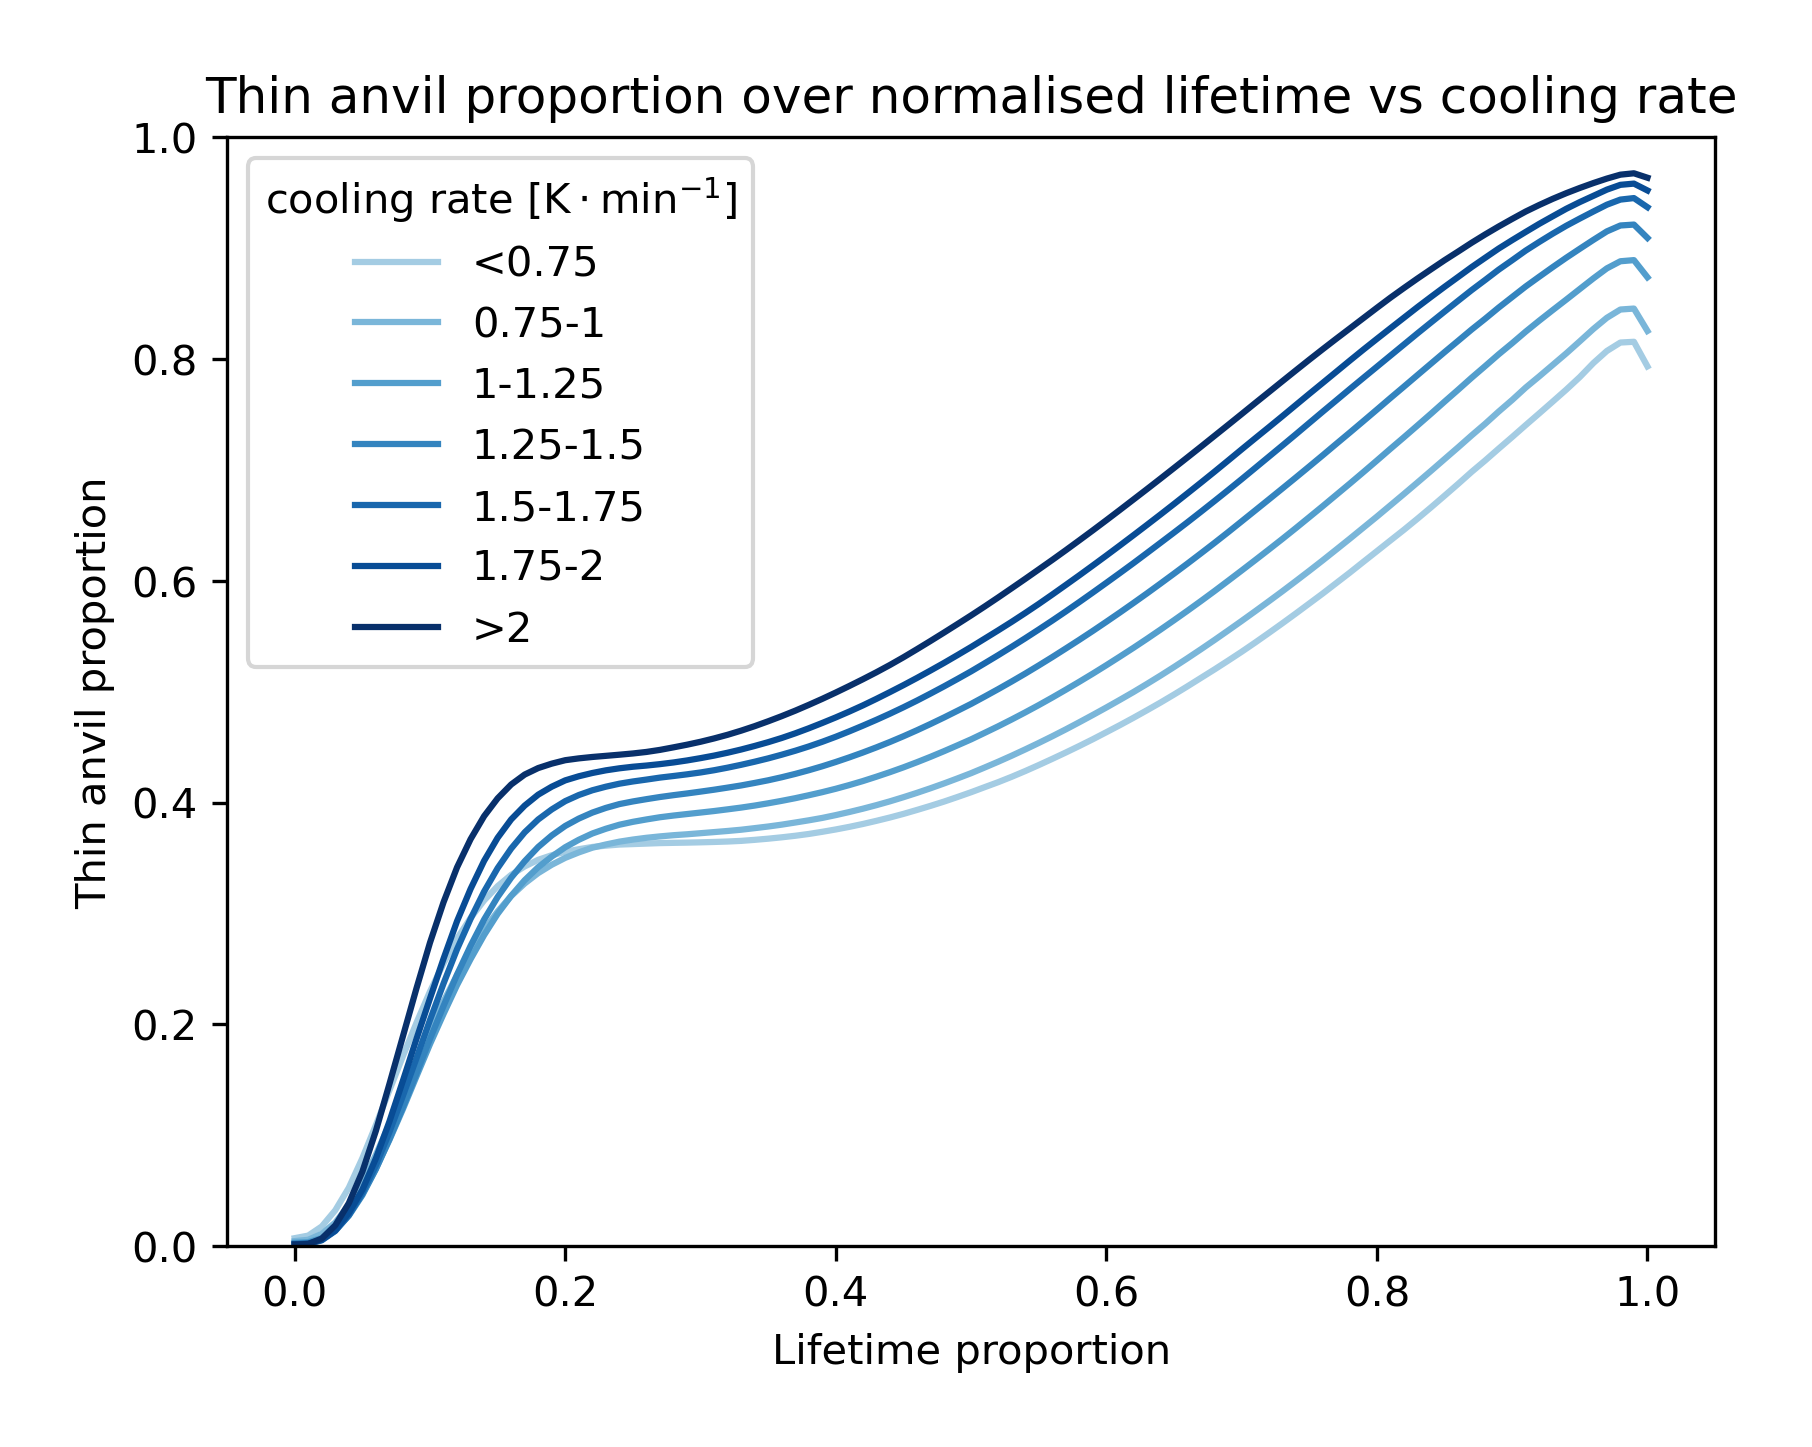
\includegraphics[width=0.75\textwidth]{figures/chapter3_13.png}
    \caption[
    Mean thin anvil proportion for composites of anvil area of normalised lifetime categorised by the cooling rate of their initial cores.
    ]{
    Mean thin anvil proportion for composites of anvil area of normalised lifetime categorised by the cooling rate of their initial cores. More intense core cooling rates are shown by the darker blue lines.
    }
    \label{fig:cooling_rate_composite}
\end{figure}


Figure~\ref{fig:cooling_rate_composite} shows composites of the thin anvil fraction for \acrshort{dcc}s grouped by core cooling rate, with larger cooling rates shown in darker shades of blue.
Each of the composites has a similar shape to the evolution of thin anvil fraction shown in fig.~\ref{fig:composite_example}\,b; an initial rapid increase as the anvil develops, a plateau during the maturing stage and a continual increase as the anvil dissipates.
Two sections of the lifecycle show divergence in the thin anvil fraction with core cooling rate.
Firstly, more intense cores produce a higher thin anvil fraction during the developing phase.
This difference in thin anvil fraction is then maintained throughout the mature phase.
Secondly, the thin anvil fraction further diverges during the dissipating phase, with the anvils originating from more intense cores having a larger increase in thin anvil fraction.
This difference during the dissipating stage may be related to the difference in the thin anvil lifetime seen previously.


%f
\begin{figure}[tp]
    \centering
    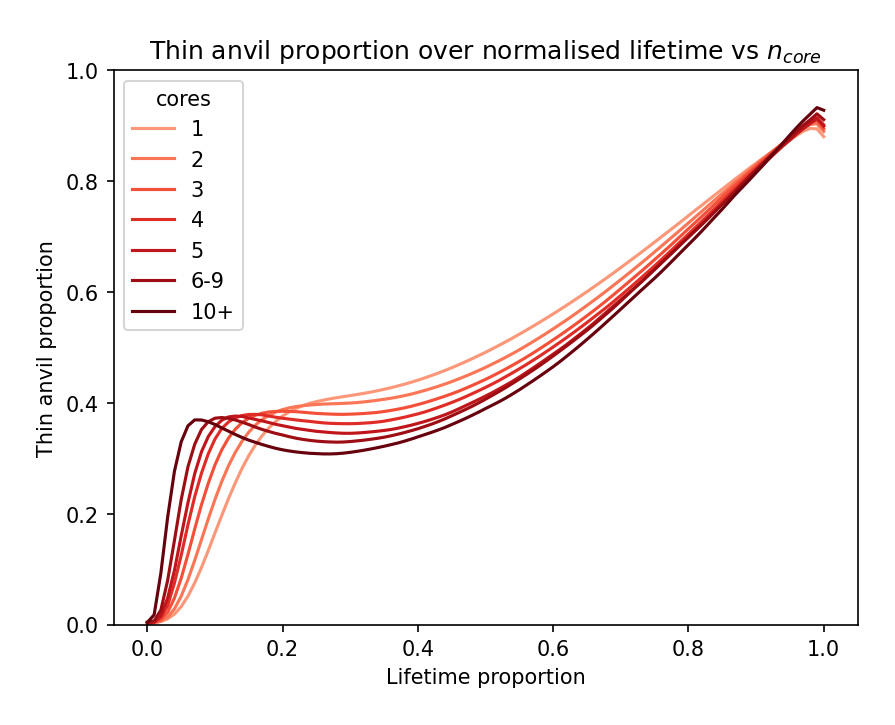
\includegraphics[width=0.75\textwidth]{figures/chapter3_14.png}
    \caption[
    Mean thin anvil proportion for composites of anvil area of normalised lifetime categorised by the number of cores
    ]{
    Mean thin anvil proportion for composites of anvil area of normalised lifetime categorised by the number of cores. Anvils with a larger number of cores are shown by the darker red lines.
    }
    \label{fig:number_of_cores_composite}
\end{figure}

Figure~\ref{fig:number_of_cores_composite} compares how the mean thin anvil fraction changes for composites grouped by the number of cores.
The composites with a greater number of cores are shown by the darker shades of red.
In contrast to fig.~\ref{fig:cooling_rate_composite}, a difference from the typical shape of the thin anvil fraction established in fig.~\ref{fig:composite_example} is seen for more organised \acrshort{dcc}s.
At the end of the initial development phase of the anvil there is a similar thin anvil fraction of around 0.4 across all cases.
While the more organised \acrshort{dcc}s reach this point faster, this is simply due to the initial anvil time making up a smaller proportion of the total lifetime due to the latter's increase with convective organisation.

After the initial development of the anvil, there is a divergence in the thin anvil fraction during the later growing stage and the mature stage.
For the most organised \acrshort{dcc}s, there is a reduction in the thin anvil fraction during this period, indicating that the continuous, organised convection from multiple convective cores leads to a thickening of the anvil.
This difference in thin anvil remains into the dissipating stage, however the composites all converge to a similar fraction by the end of their lifecycles.

The investigation of changes in thin anvil fraction over \acrshort{dcc} lifecycle using composites reveals further complexity to the response of thin anvil structure to convective processes.
Not only do changes in intensity and organisation have contrasting effects on the net thin anvil fraction and the lifecycle, they also impact the anvil structure at different stages throughout the \acrshort{dcc} lifetime.
The timing of when differences in structure are seen may help investigate the processes through which they occur.


\section{Summary}

Deep convective anvil clouds have a characteristic \acrshort{toa} \acrshort{cre} that is near neutral \citep{hartmann_tropical_2016}.
Anvils are, however, not homogeneous objects, and exhibit structures that transition from thick near the convective cores to thin, detrained cirrus further away.
The tendency of reflectivity to reduce faster than emissivity with reducing cloud optical thickness, combined with the large \acrshort{sw} and \acrshort{lw} \acrshort{cre} of anvils, means that the \acrshort{cre} varies widely with changing thickness \citep{berry_cloud_2014}.
Despite this, the response of anvil optical properties to climate change remains largely uncertain, in part due to the lack of data connecting the behaviour of convective cores and anvils \cite{gasparini_opinion_2023}.

Previous studies have found that the fraction of thin anvil increases with increasing convective intensity \citep{protopapadaki_upper_2017, takahashi_relationships_2017}.
These studies were performed using sun-synchronous polar-orbiting satellite data, and so could not resolve changes across the lifecycle of \acrshort{dcc}s.
With the dataset of tracked \acrshort{dcc} cores and anvils, changes in the convective properties can be related to changes in structure observed over the entire anvil lifecycle.

Using the initial core cooling rate and number of cores as proxies for the intensity and organisation of convection respectively, a similar increase in thin anvil fraction is found with increasing intensity, but a decrease with increasing organisation.
These relationships are found to be robust across a wide range of convective environments.
Contrasting impacts on \acrshort{dcc} lifecycle are also found as a result of both processes.
In more intense \acrshort{dcc}s, there is a reduction in the length of the growing phase and an increase in the thin anvil lifetime, whereas the opposite occurs in more organised cases.
These corresponding changes in lifecycle indicate that the thin anvil fraction cannot be determined from single snapshots alone.

By analysing composites of the change in thin anvil fraction over the \acrshort{dcc} lifecycle, impacts of intensity and organisation are apparent at different periods during the \acrshort{dcc} lifetime.
The timing of these changes also indicates which processes may be impacting the anvil structure in each case.
For the more intense convection, there is an increase in the thin anvil fraction during the initial formation of the anvil, which is then maintained as the anvil matures.
Studies of anvil evolution in high-resolution convective resolving models have shown that, during the initial growth of the anvil, before the development of compensating downdrafts within the core, the divergence of the anvil is directly linked to the updraft velocities within the core \citep{senf_highresolution_2018}.
After the formation of compensating downdrafts after around 15--20 minutes, this connection is broken which may explain why this difference only occurs during the very early formation of the anvil.

A second period of increasing divergence in thin anvil fraction is seen during the dissipating stage of the \acrshort{dcc}s.
As this occurs after the end of the convective updrafts, it cannot be related directly to the convective processes but instead to their impact on the anvil properties.
Over the lifetime of anvils, radiative heating of the cloud base and cooling of the cloud top result in circulations within the anvil cloud which have a thinning effect \citep{gasparini_what_2019}.
Once the anvil is sufficiently thin however (with optical depths around 1), these radiatively driven circulations cease and instead the remainder of the dissipation occurs due to the sedimentation and sublimation of the remaining thin cirrus \citep{sokol_tropical_2020}.
At the higher altitudes and colder temperatures of the anvils produced by more intense convection these processes are substantially slower \citep{seeley_formation_2019}, potentially resulting in larger extents and lifetimes for the thin, but not thick, anvil.

For more organised \acrshort{dcc}s a reduction in the thin anvil fraction is observed not during the initial anvil formation but during the subsequent growing and maturing period of the anvil.
Unlike isolated systems, organised \acrshort{dcc}s involve the continuous development of new convective cores throughout most of the lifecycle of the more organised \acrshort{dcc}s.
It is possible that the thickening is a result of the mesoscale circulations associated with large, organised \acrshort{mcs}s, which transports additional moisture directly into the anvil where it increases the cloud water content at high levels.  
Alternatively, convective aggregation may result in moister environments surrounding the cores of these organised \acrshort{dcc}s, slowing the dissipation of the thick anvil, and also drying the surrounding regions resulting in faster decay of the thin anvil further from the core.
The convergence of the thin anvil fraction during the dissipating phase of \acrshort{dcc}s is indicative of the characteristic decay patterns seen in convective anvils across scales \citep{roca_simple_2017, elsaesser_simple_2022}.

Further investigation of how these processes impact anvil structure and lifecycle may be difficult due to the lack of time-resolved observational data that can measure these processes.
The use of modelling, including both convective resolving models and more idealised experiments, may provide a route to isolate the impacts of each process on \acrshort{dcc} evolution \citep{gasparini_diurnal_2022}.

The final element to consider is how these observed changes in anvil structure may impact the anvil \acrshort{cre}.
Considering the thin anvil fraction alone, it could be expected that more intense \acrshort{dcc}s are more warming due to their thinner structure, and vice versa for more organised convection.
However, this neglects other factors relevant to anvil \acrshort{cre} that are also impacted by convective processes.
Both convective intensity and organisation affect the temperature of anvil clouds, resulting in a warming effect for increases in both.
Furthermore, the observed changes in the lifecycle and the timing of the maximum extent of the thick anvil within the \acrshort{dcc} lifetime may impact the \acrshort{sw} \acrshort{cre}, particularly over land due to the pronounced diurnal cycle of convection.
Observational studies have shown a link between increasing convective organisation and domain mean \acrshort{toa} cooling \citep{bony_observed_2020}.
While this has traditionally been explained as a result of greater clear sky \acrshort{lw} emissions to space \citep{bony_thermodynamic_2016}, this could also result from the response of anvil \acrshort{cre} to changes in structure.
